\chapter{Supplementary Data Figures} % Main appendix title

\label{AppendixB} 

\begin{figure}
  \centering
  	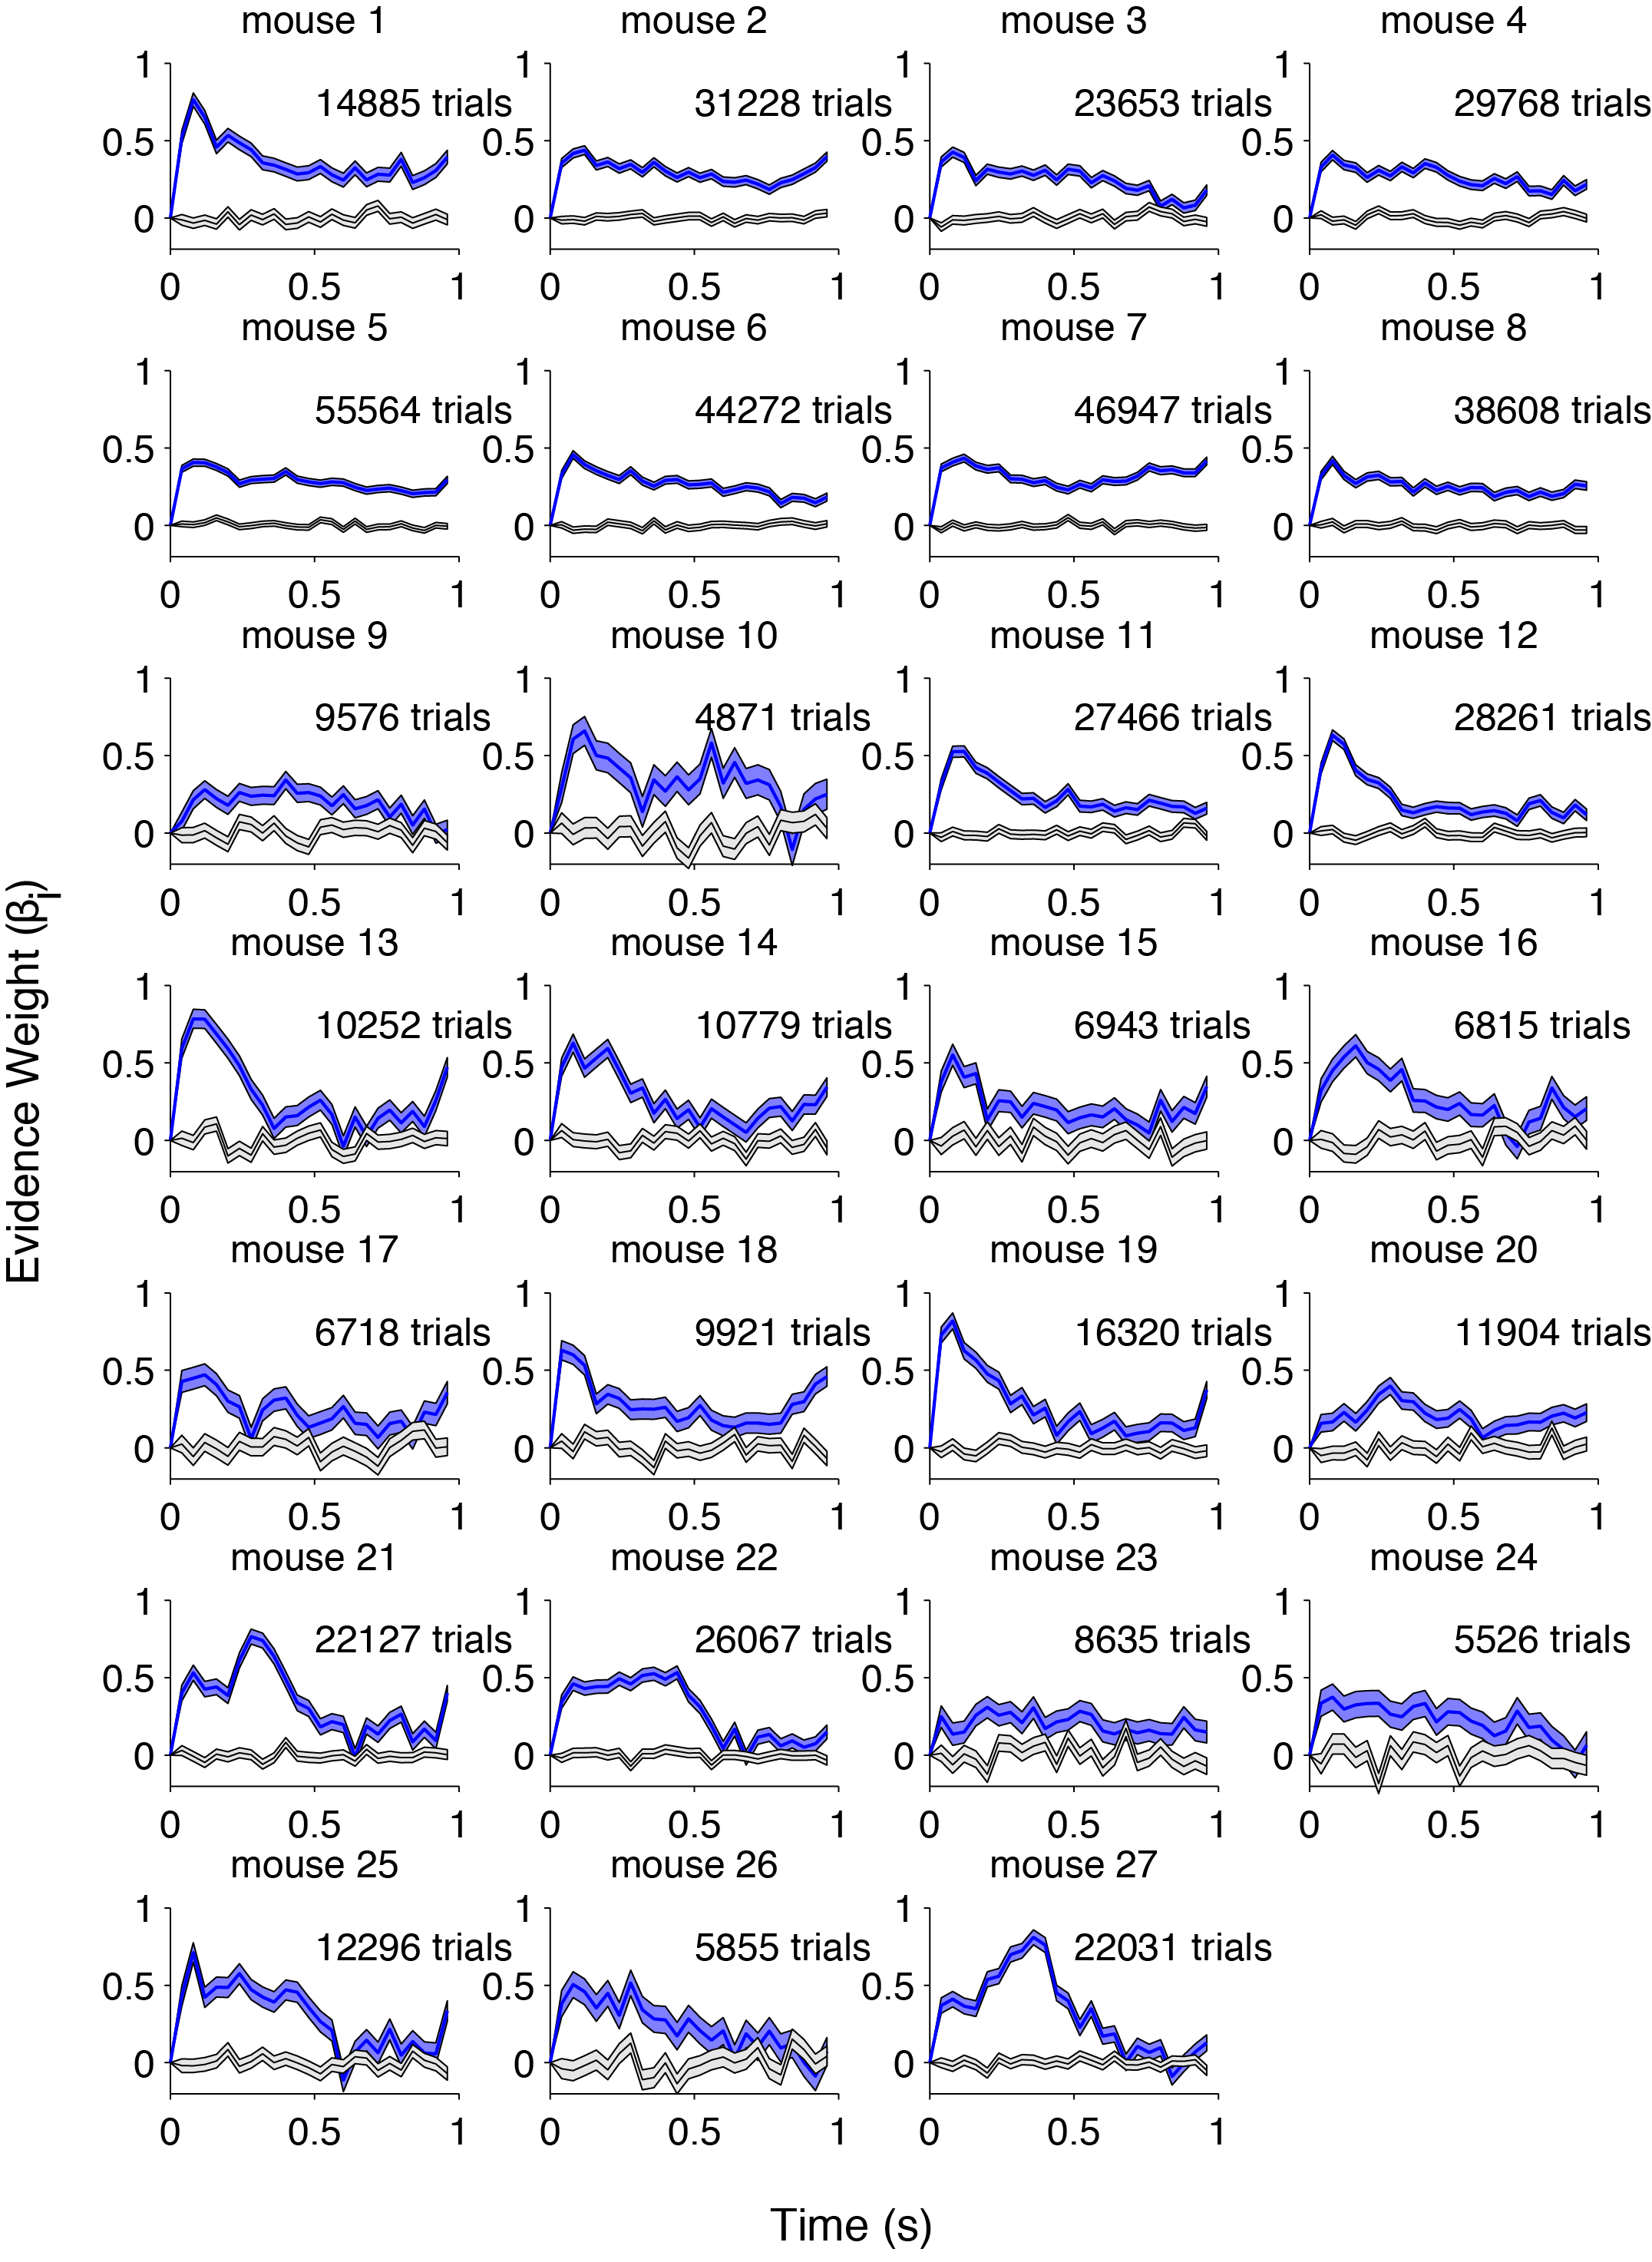
\includegraphics[width=\textwidth,height=\textheight,keepaspectratio]{Figures/chapter2/psychKernel_individualmice.png}
  \caption[Psychophysical Kernels of Individual Mice]{\textbf{Psychophysical Kernels of Individual Mice}. Data (blue) and shuffle control (gray). Shaded areas represent standard error of estimated coefficients.}
   \label{fig:allkernels2}
\end{figure}
%--------------------------------------------------------------------------

\begin{figure}
  \centering
  	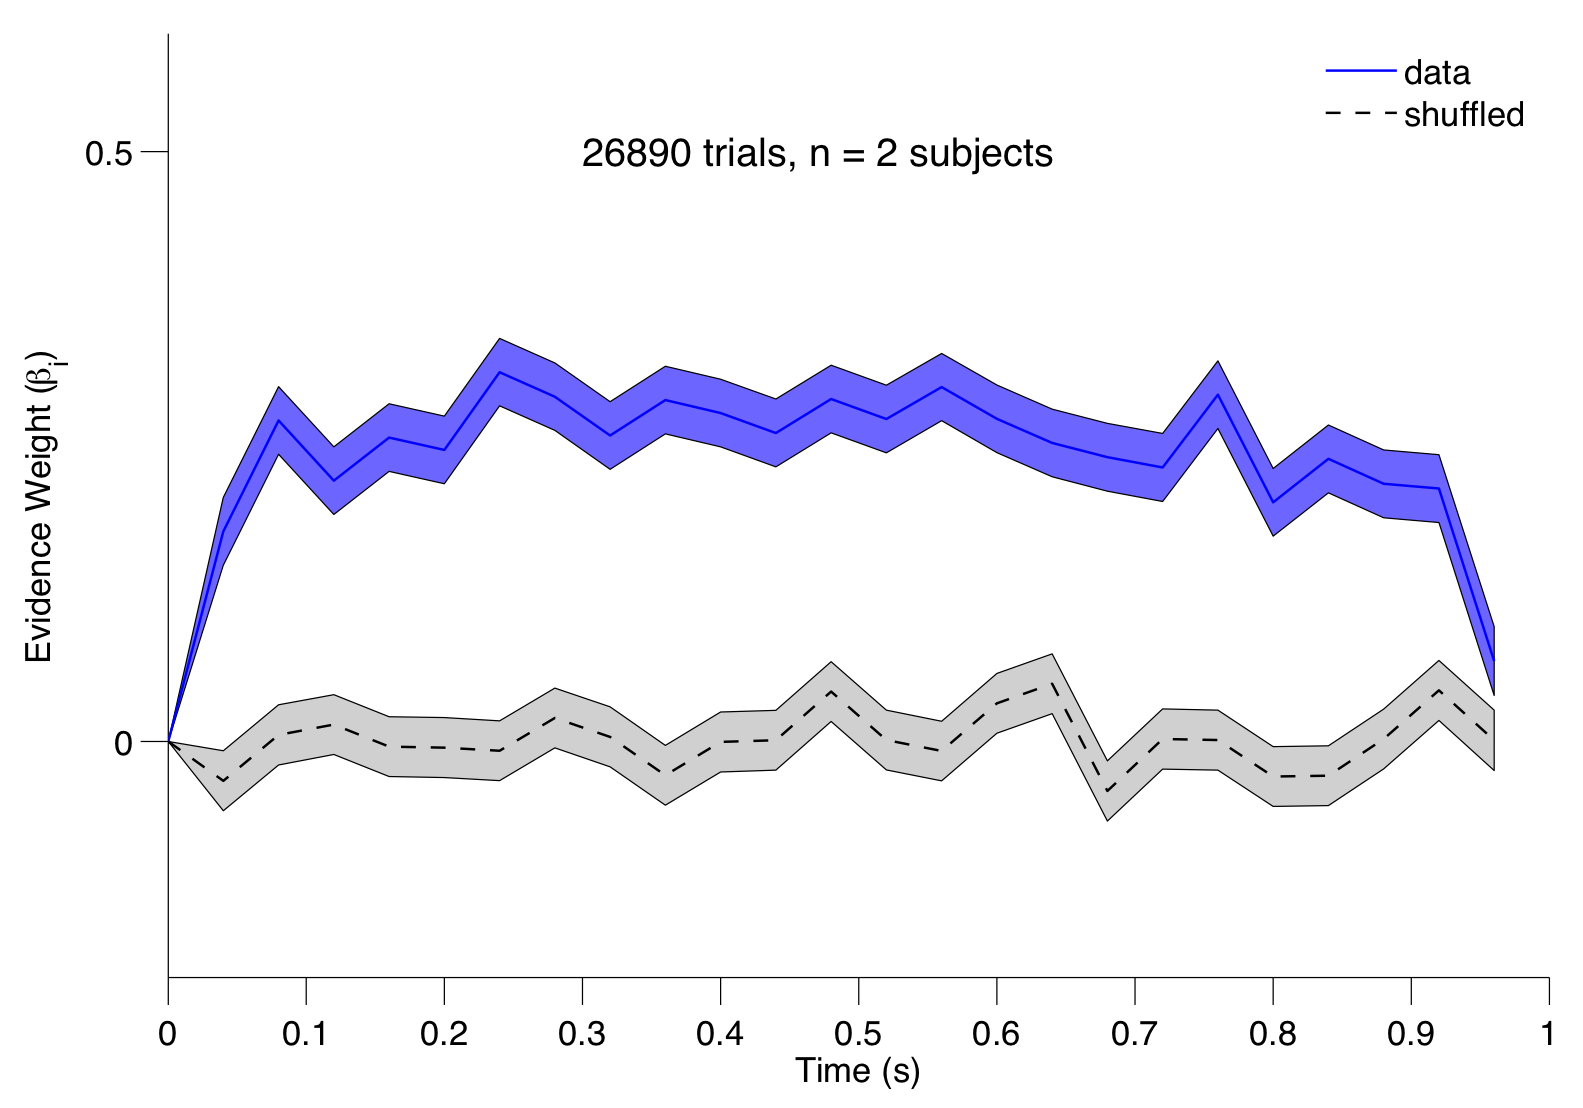
\includegraphics[width=\textwidth,height=\textheight,keepaspectratio]{Figures/chapter2/rat_kernel.png}
  \caption[Psychophysical Kernels of Rats Trained on Visual Flashes Task]{\textbf{Psychophysical Kernels of Rats Trained on Visual Flashes Task}. Data (blue) and shuffle control (gray). Shaded areas represent standard error of estimated coefficients.}
   \label{fig:ratkernel}
\end{figure}
%--------------------------------------------------------------------------
\begin{figure}
  \centering
   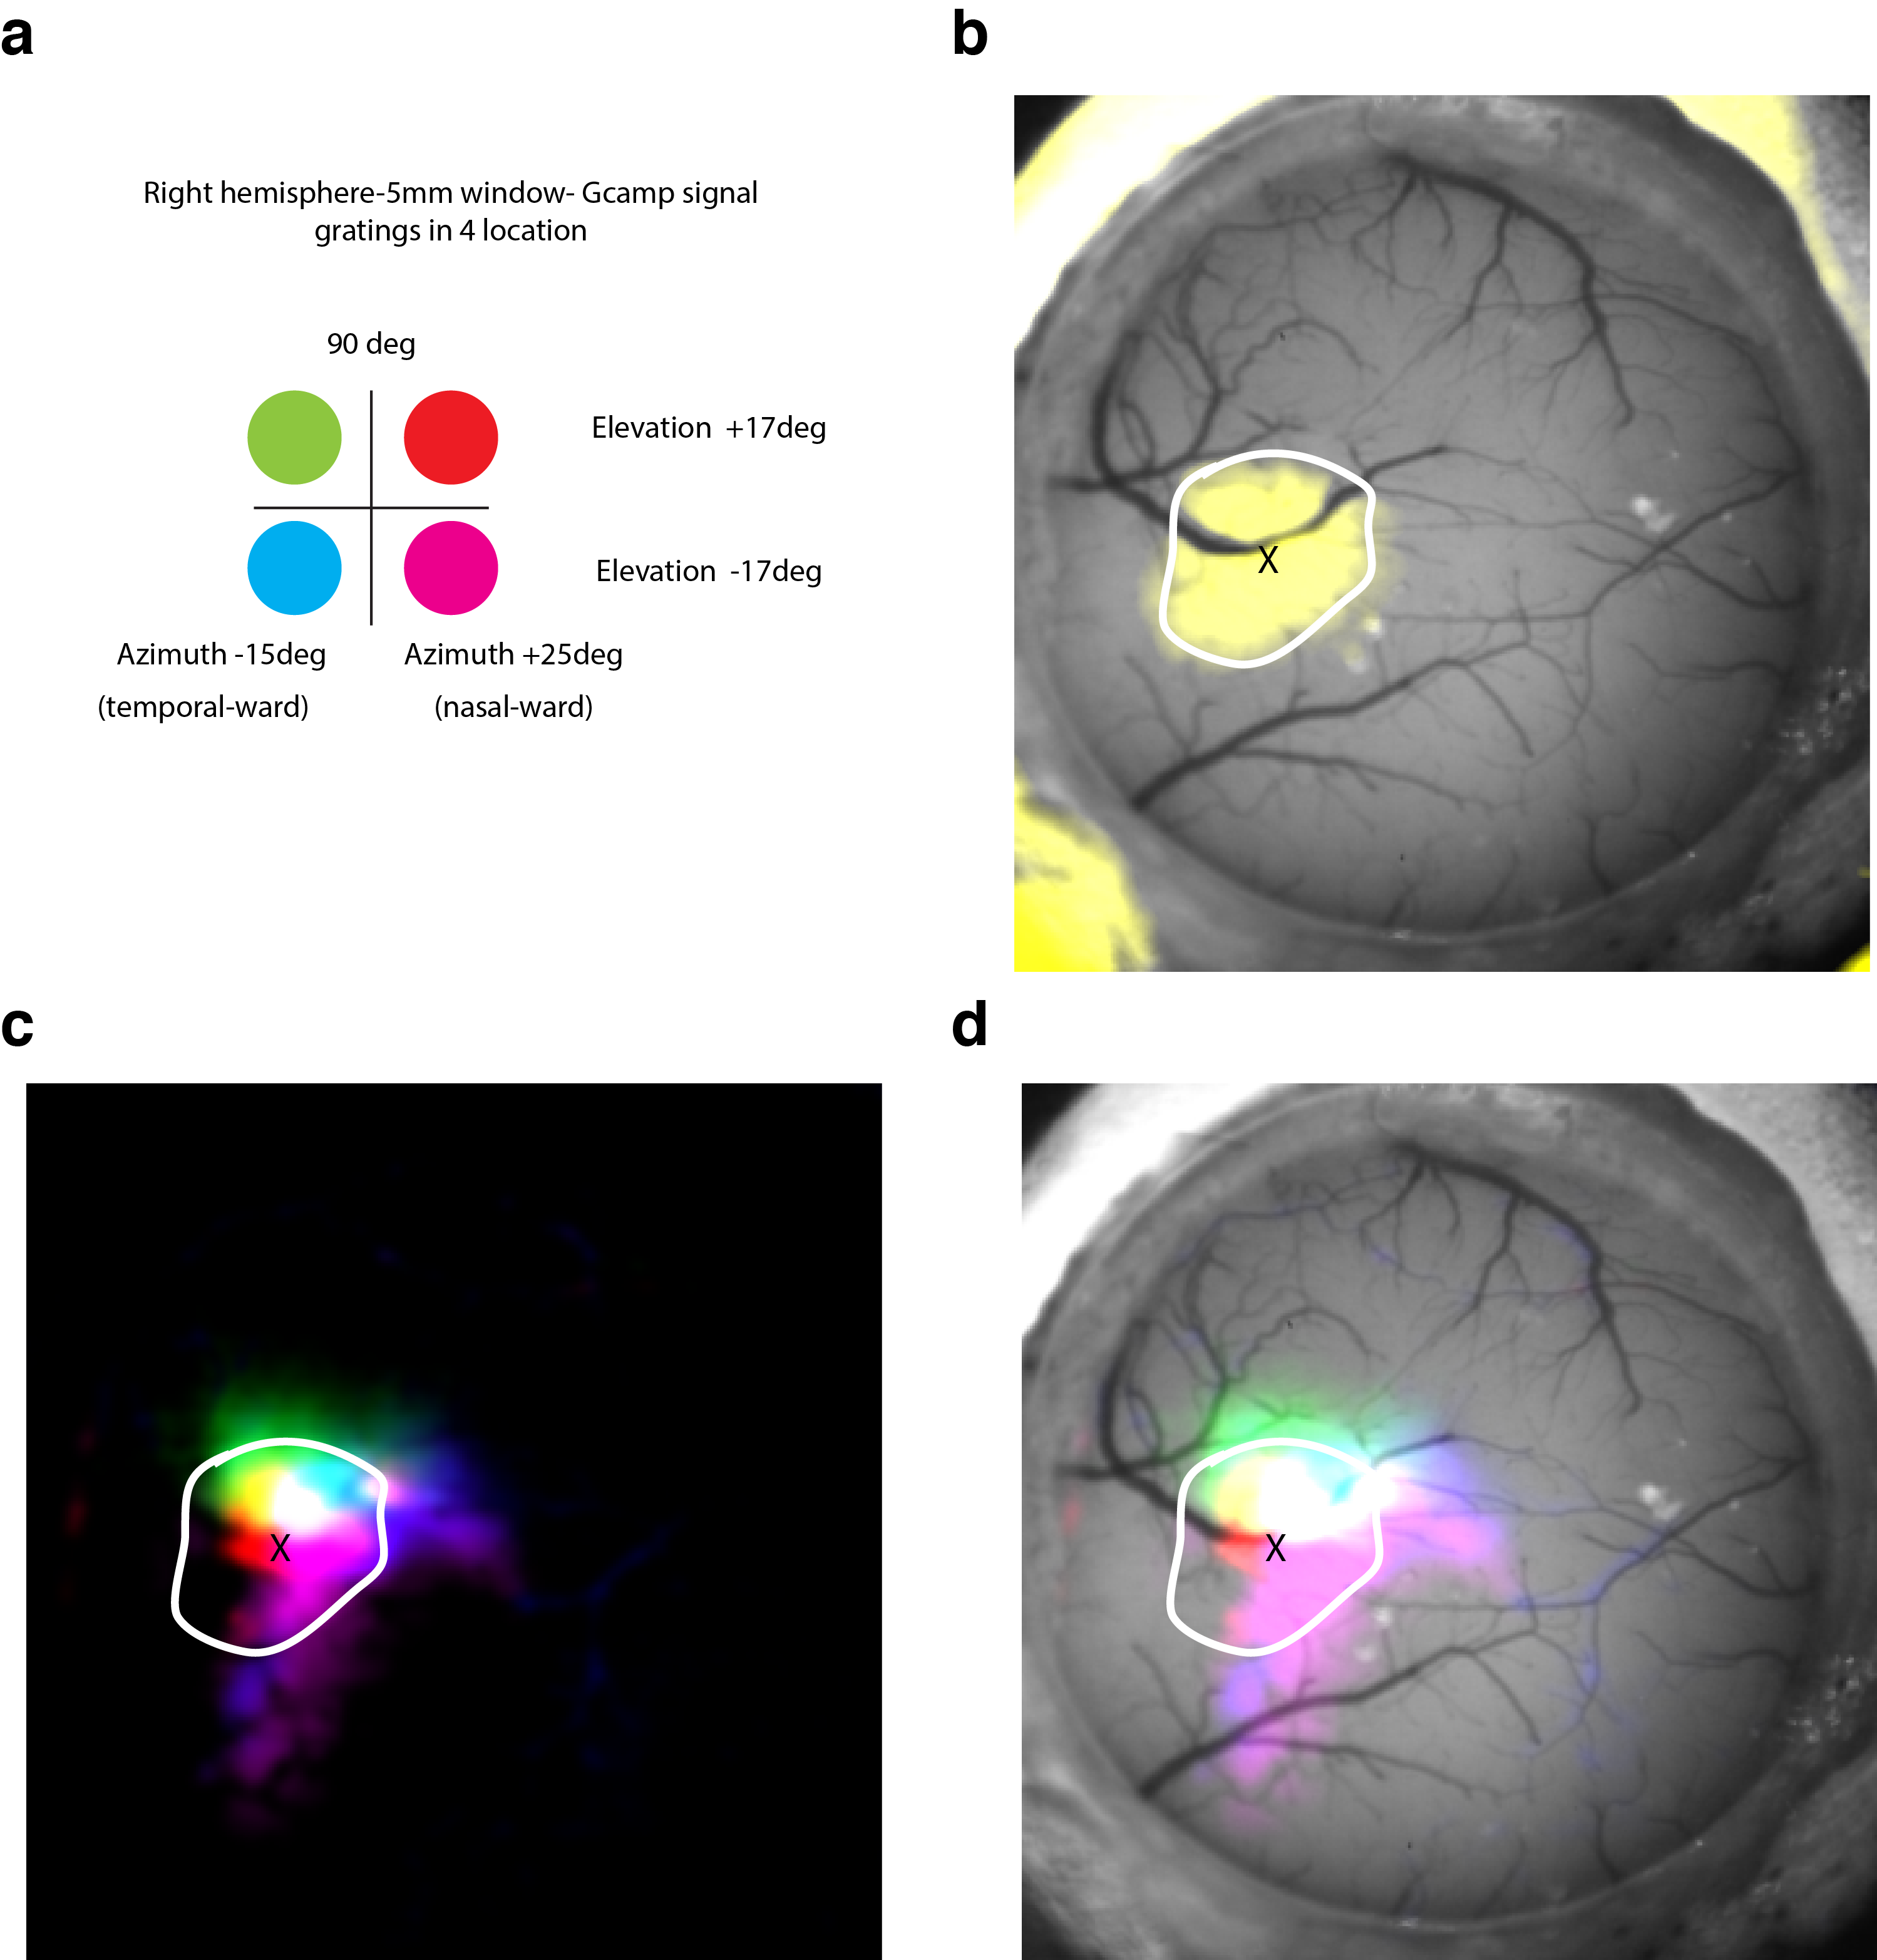
\includegraphics[width=\textwidth]{Figures/chapter4/kppc1_harvey_ppc_injections.png}
  \caption[Retinotopic Map of Stereotactic Mouse PPC]{\textbf{Retinotopic Map of Stereotactic Mouse PPC}. GCaMP6m virus was injected into stereotactic coordinates for mouse PPC (2mm posterior, 1.7mm lateral,\parencite{Harvey2012}) in the right hemisphere (a) Locations of drifting grating stimulus on monitor. The monitor was positioned at 90$\deg$ relative to the mouse (b) GCaMP6m virus expression through window (yellow). (c) Overlay of response maps from 4 stimulus locations. (d) Overlay of GCaMP6 response map with window and injection site (x).}
   \label{fig:ppcgcamp}
\end{figure}

% kPPC1 Sept06-2016
% injected aav1-syn-gcamp6m into Harvey PPC coordinates
% 2mm posterior,1.7mm lateral to bregma
% performed widefield imaging of gcamp6 signal 
%-----------------------------------------------------------------------------

\begin{figure}
  \centering
   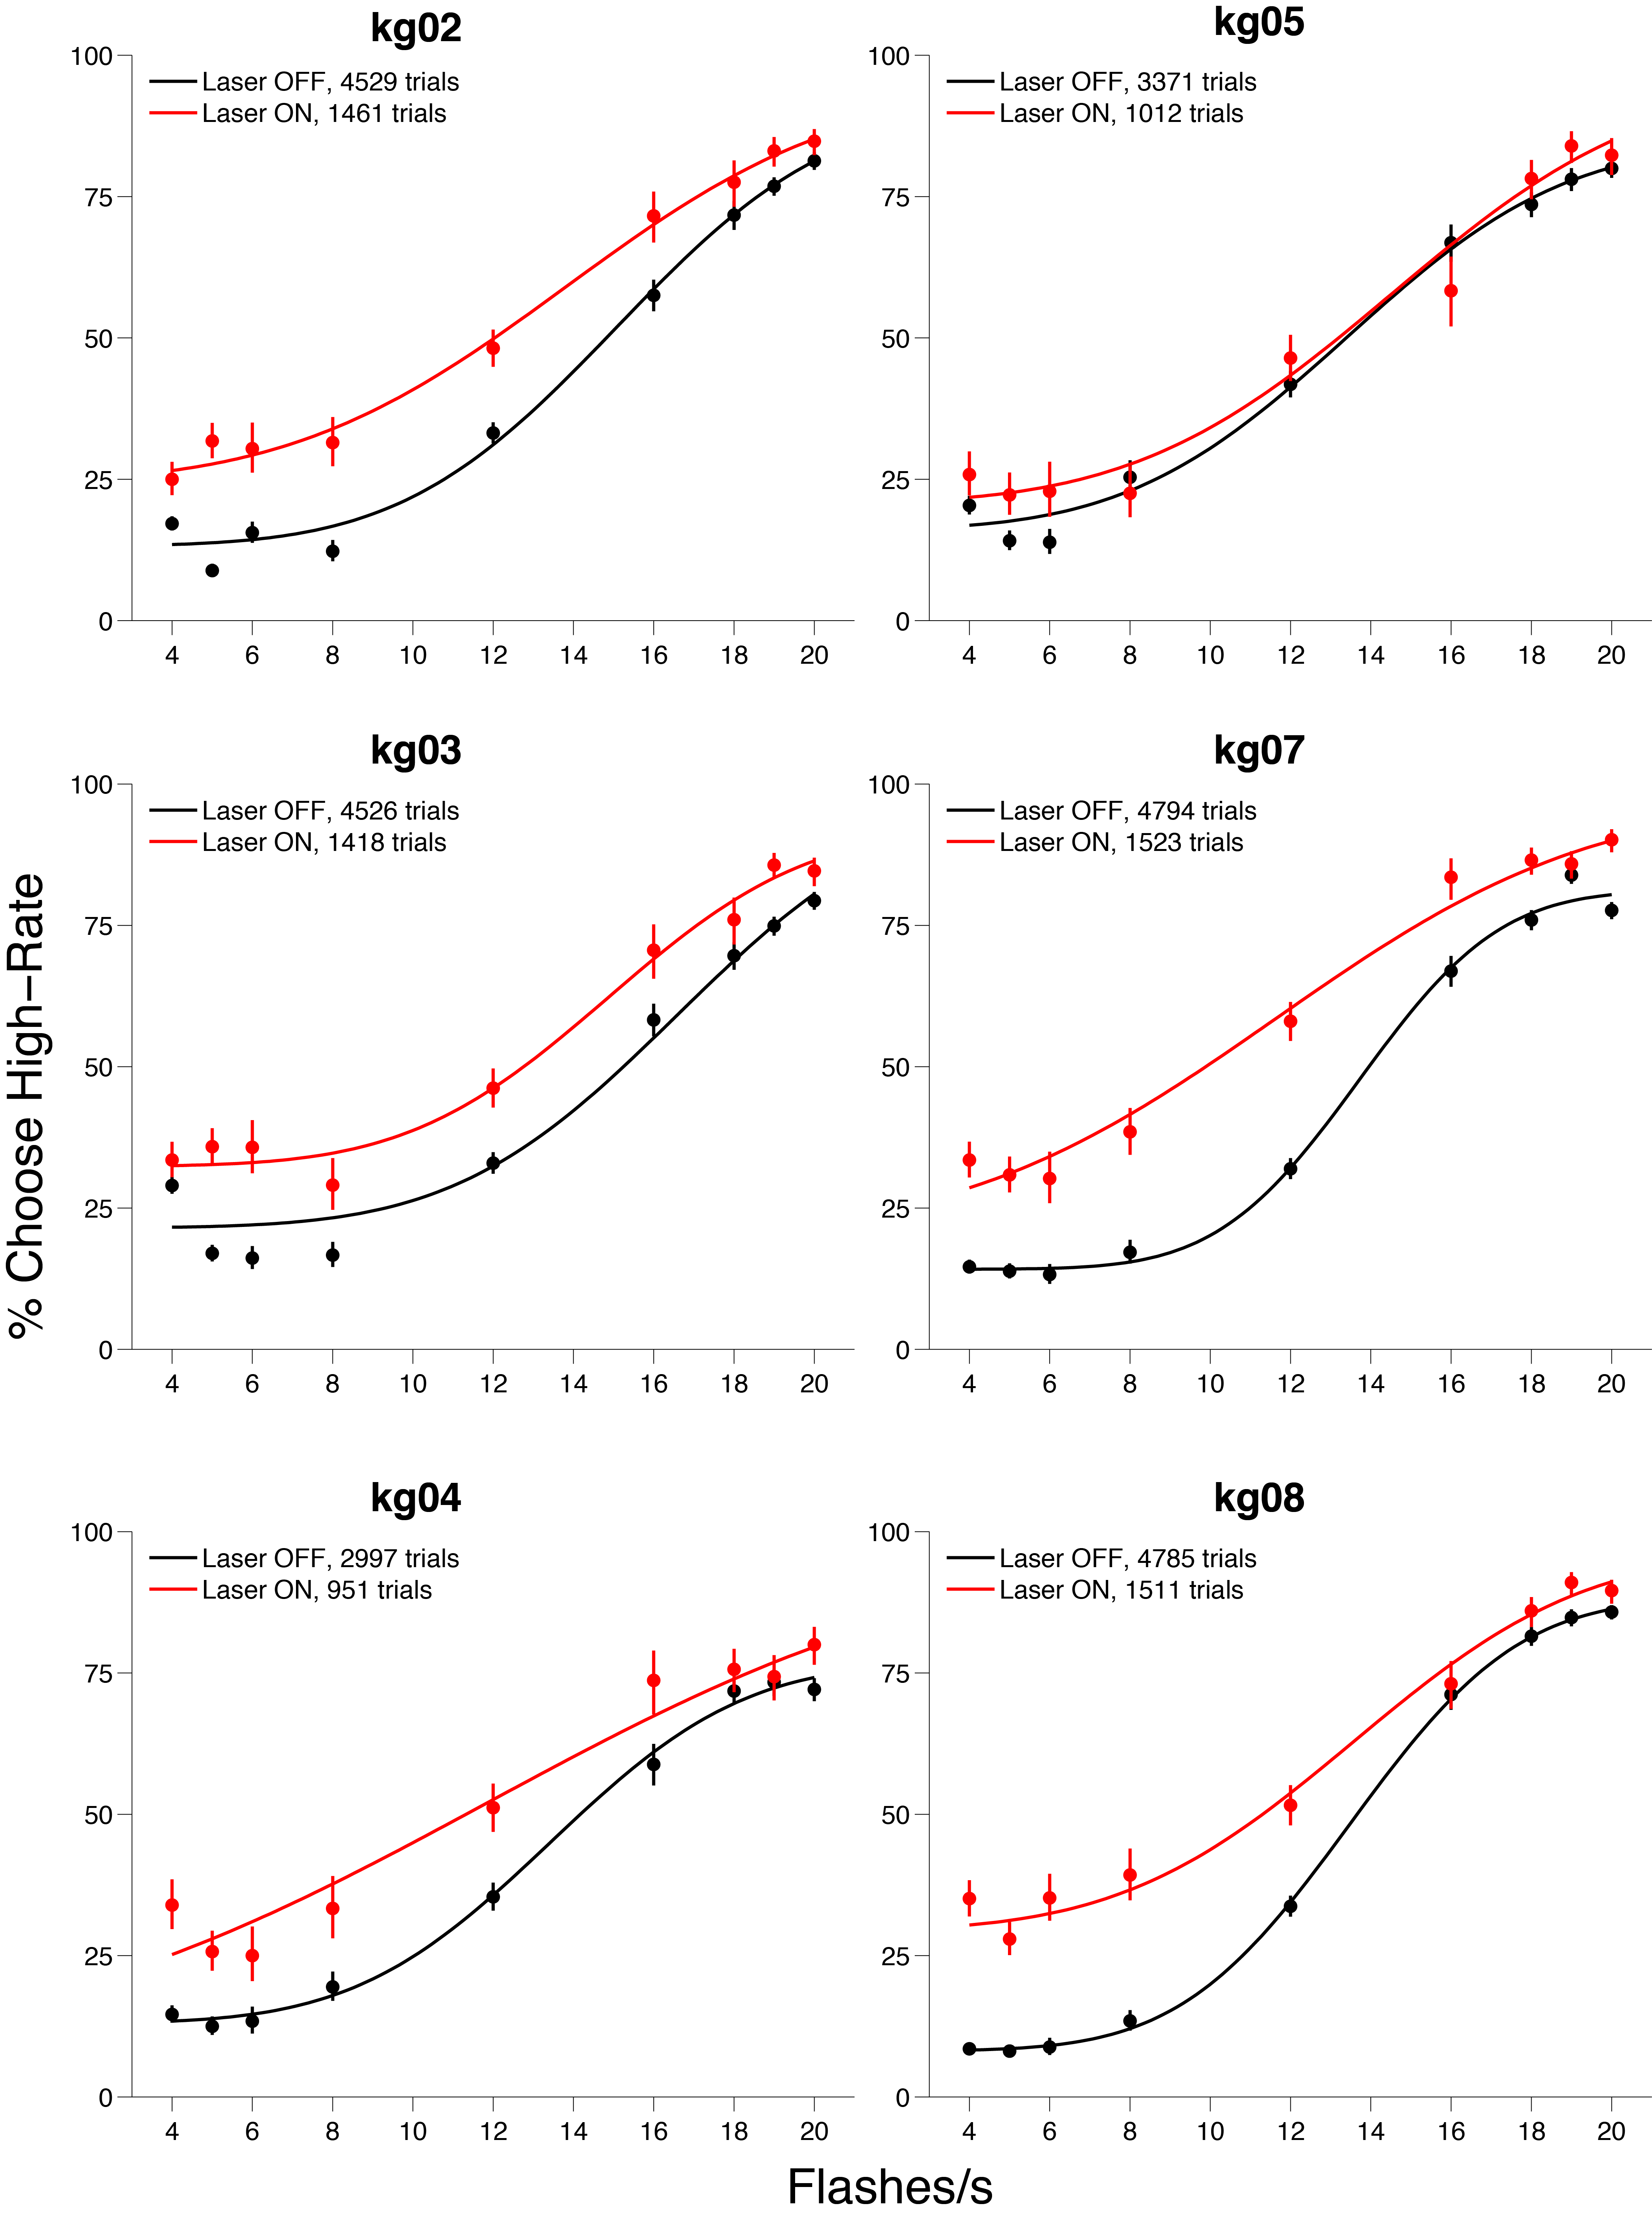
\includegraphics[width=\textwidth,height=0.8\textheight]{Figures/chapter4/jaws_AM_group1_individualPMFs.png}
  \caption[Area AM Group 1 Individual Psychophysical Data]{\textbf{Area AM Group 1 Individual Psychophysical Data}. Photoinhibition at 32 mW/mm$^{2}$. Circles represent the subject's behavioral response during laser OFF (black) and laser ON (red) trials. Solid line represents the psychometric function fit to cumulative Normal (Equation \ref{eq:normalpmf}). Error bars represent Wilson Binomial (95\%) confidence intervals. }
   \label{fig:AMgroup1individual}
\end{figure}
%-----------------------------------------------------------------------------
\begin{figure}
  \centering
   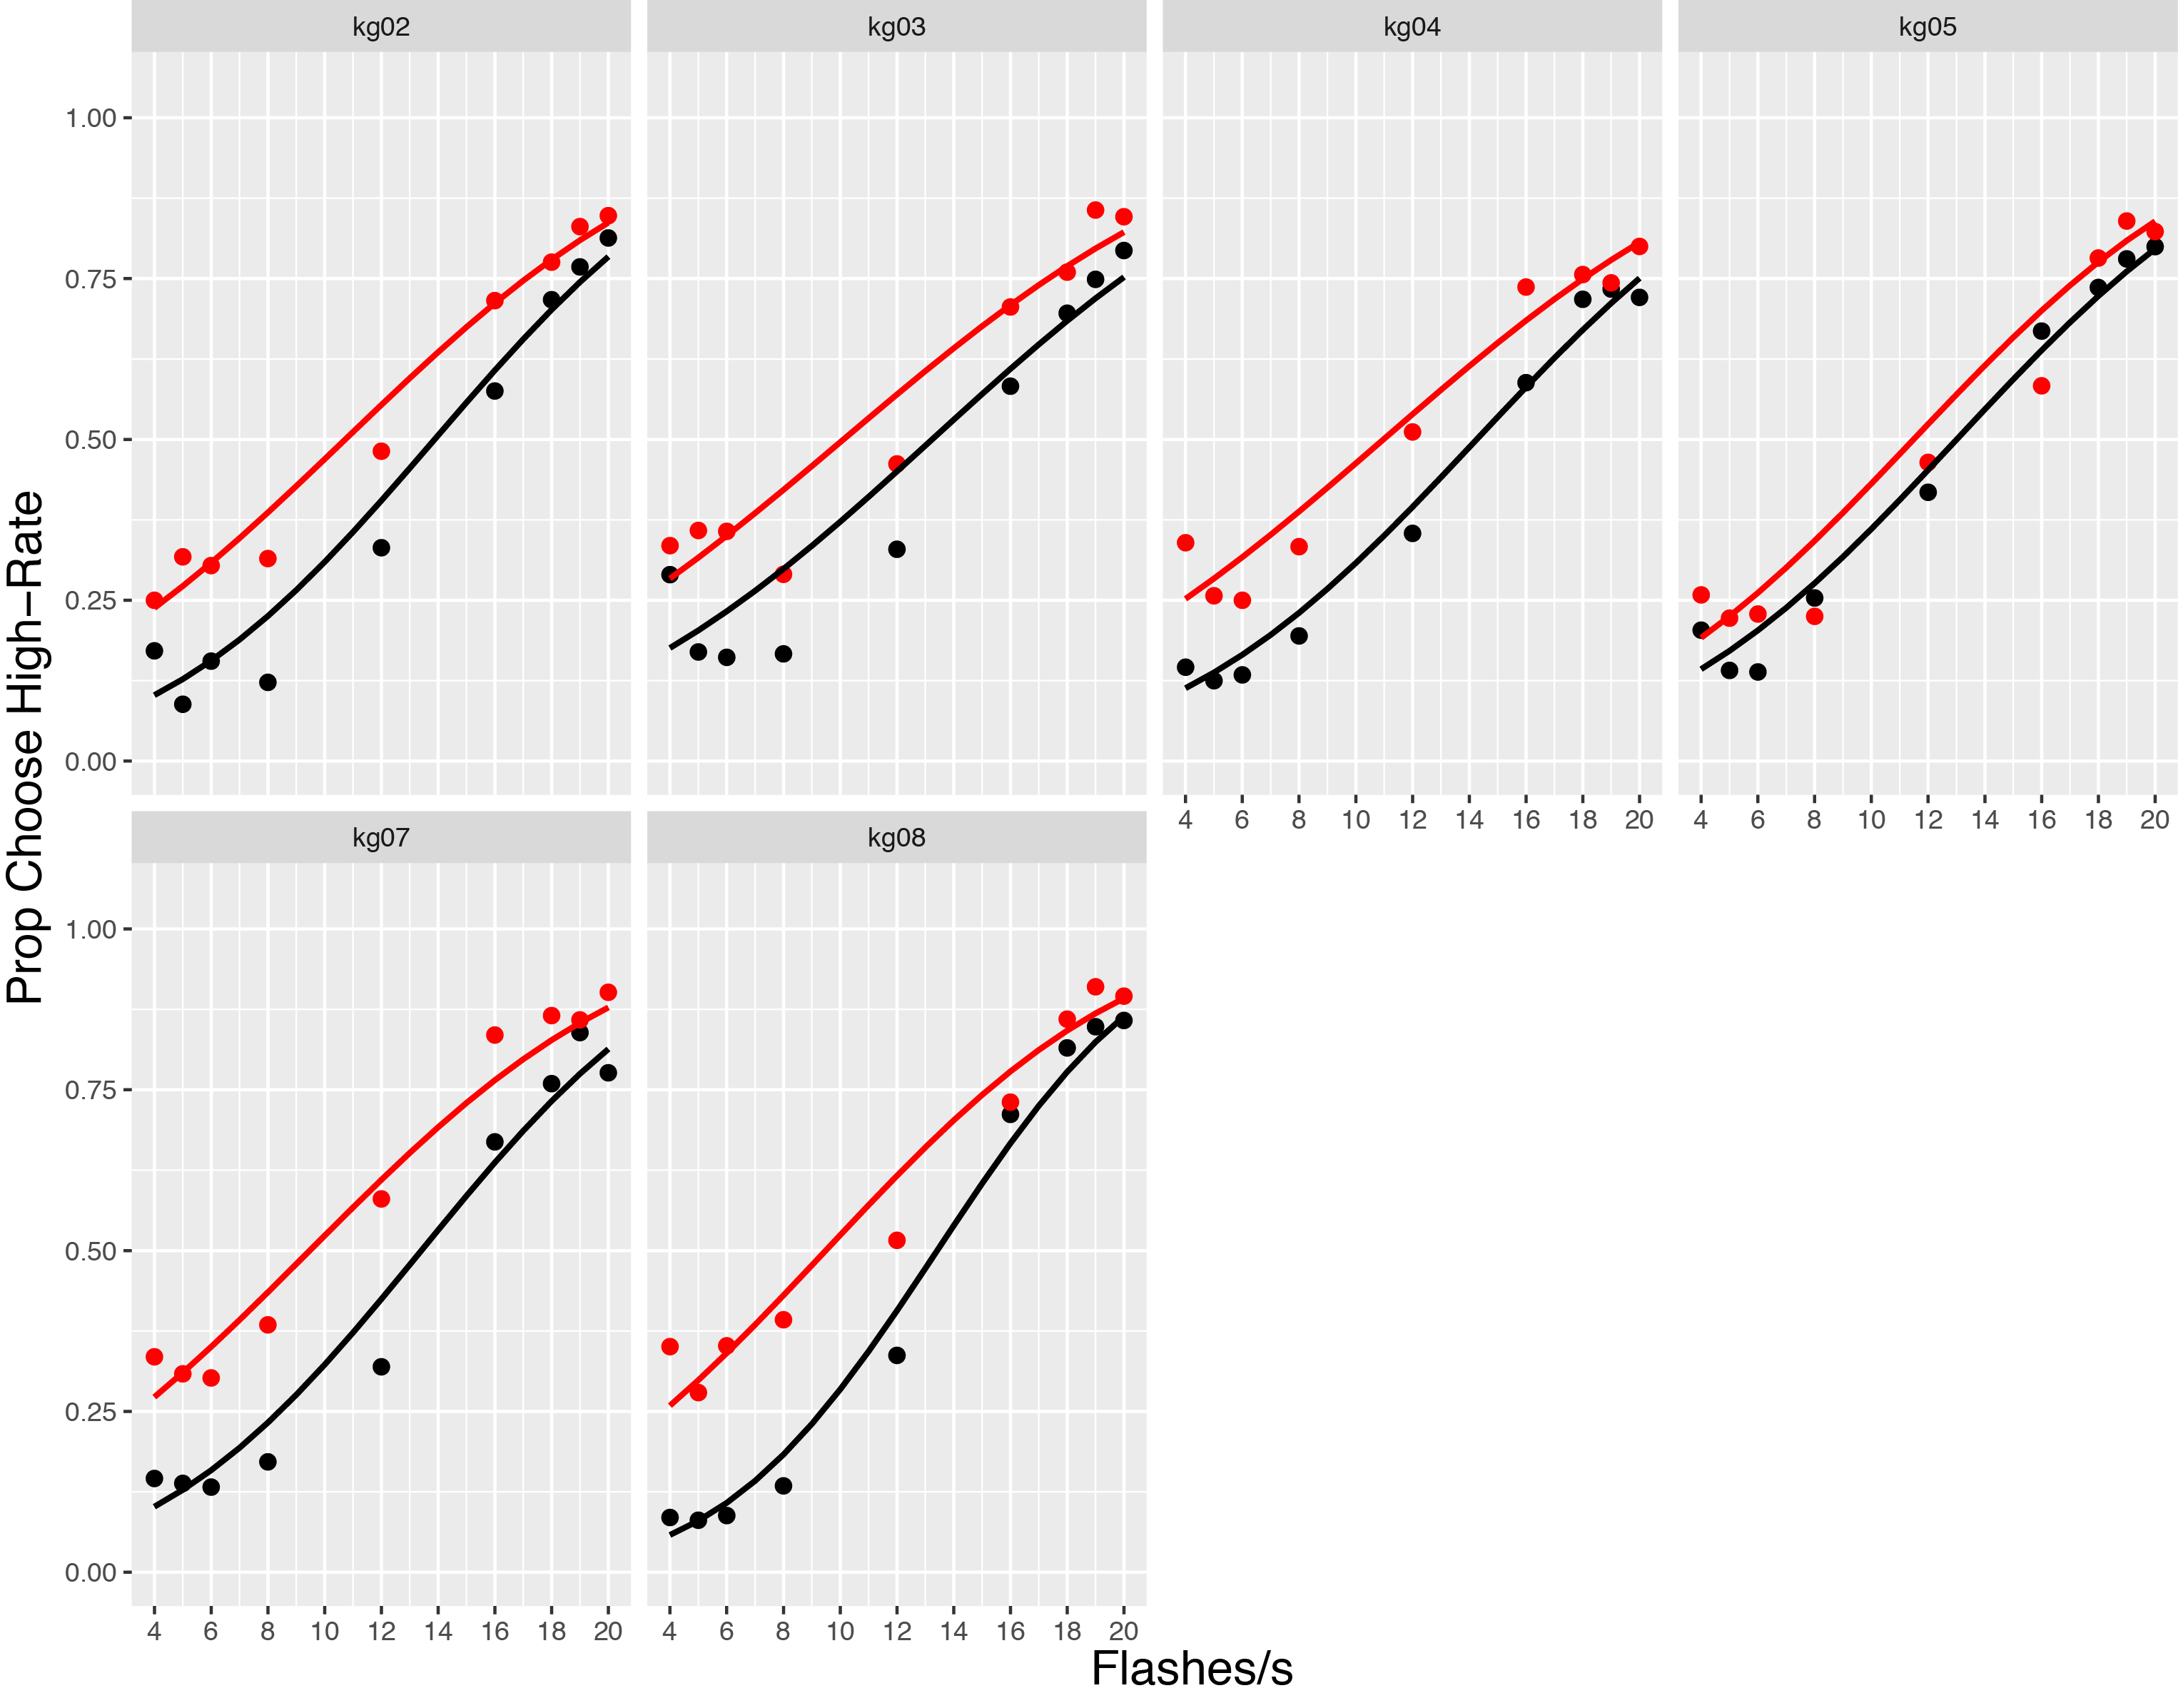
\includegraphics[width=\textwidth]{Figures/chapter4/GLMM_PMFS_32mWpermmsq_group1.png}
  \caption[Psychometric GLMM Fit - AM Group 1 - 32 mW/mm$^{2}$]{\textbf{Psychometric GLMM Fit - AM Group 1 - 32 mW/mm$^{2}$} for each mouse (n=6). Circles represent the subject's response data for laser OFF (black) and laser ON (red) conditions. The solid line represents the GLMM fit.}
   \label{fig:AMg1GLMM32}
\end{figure}
%-----------------------------------------------------------------------------
\begin{figure}
  \centering
   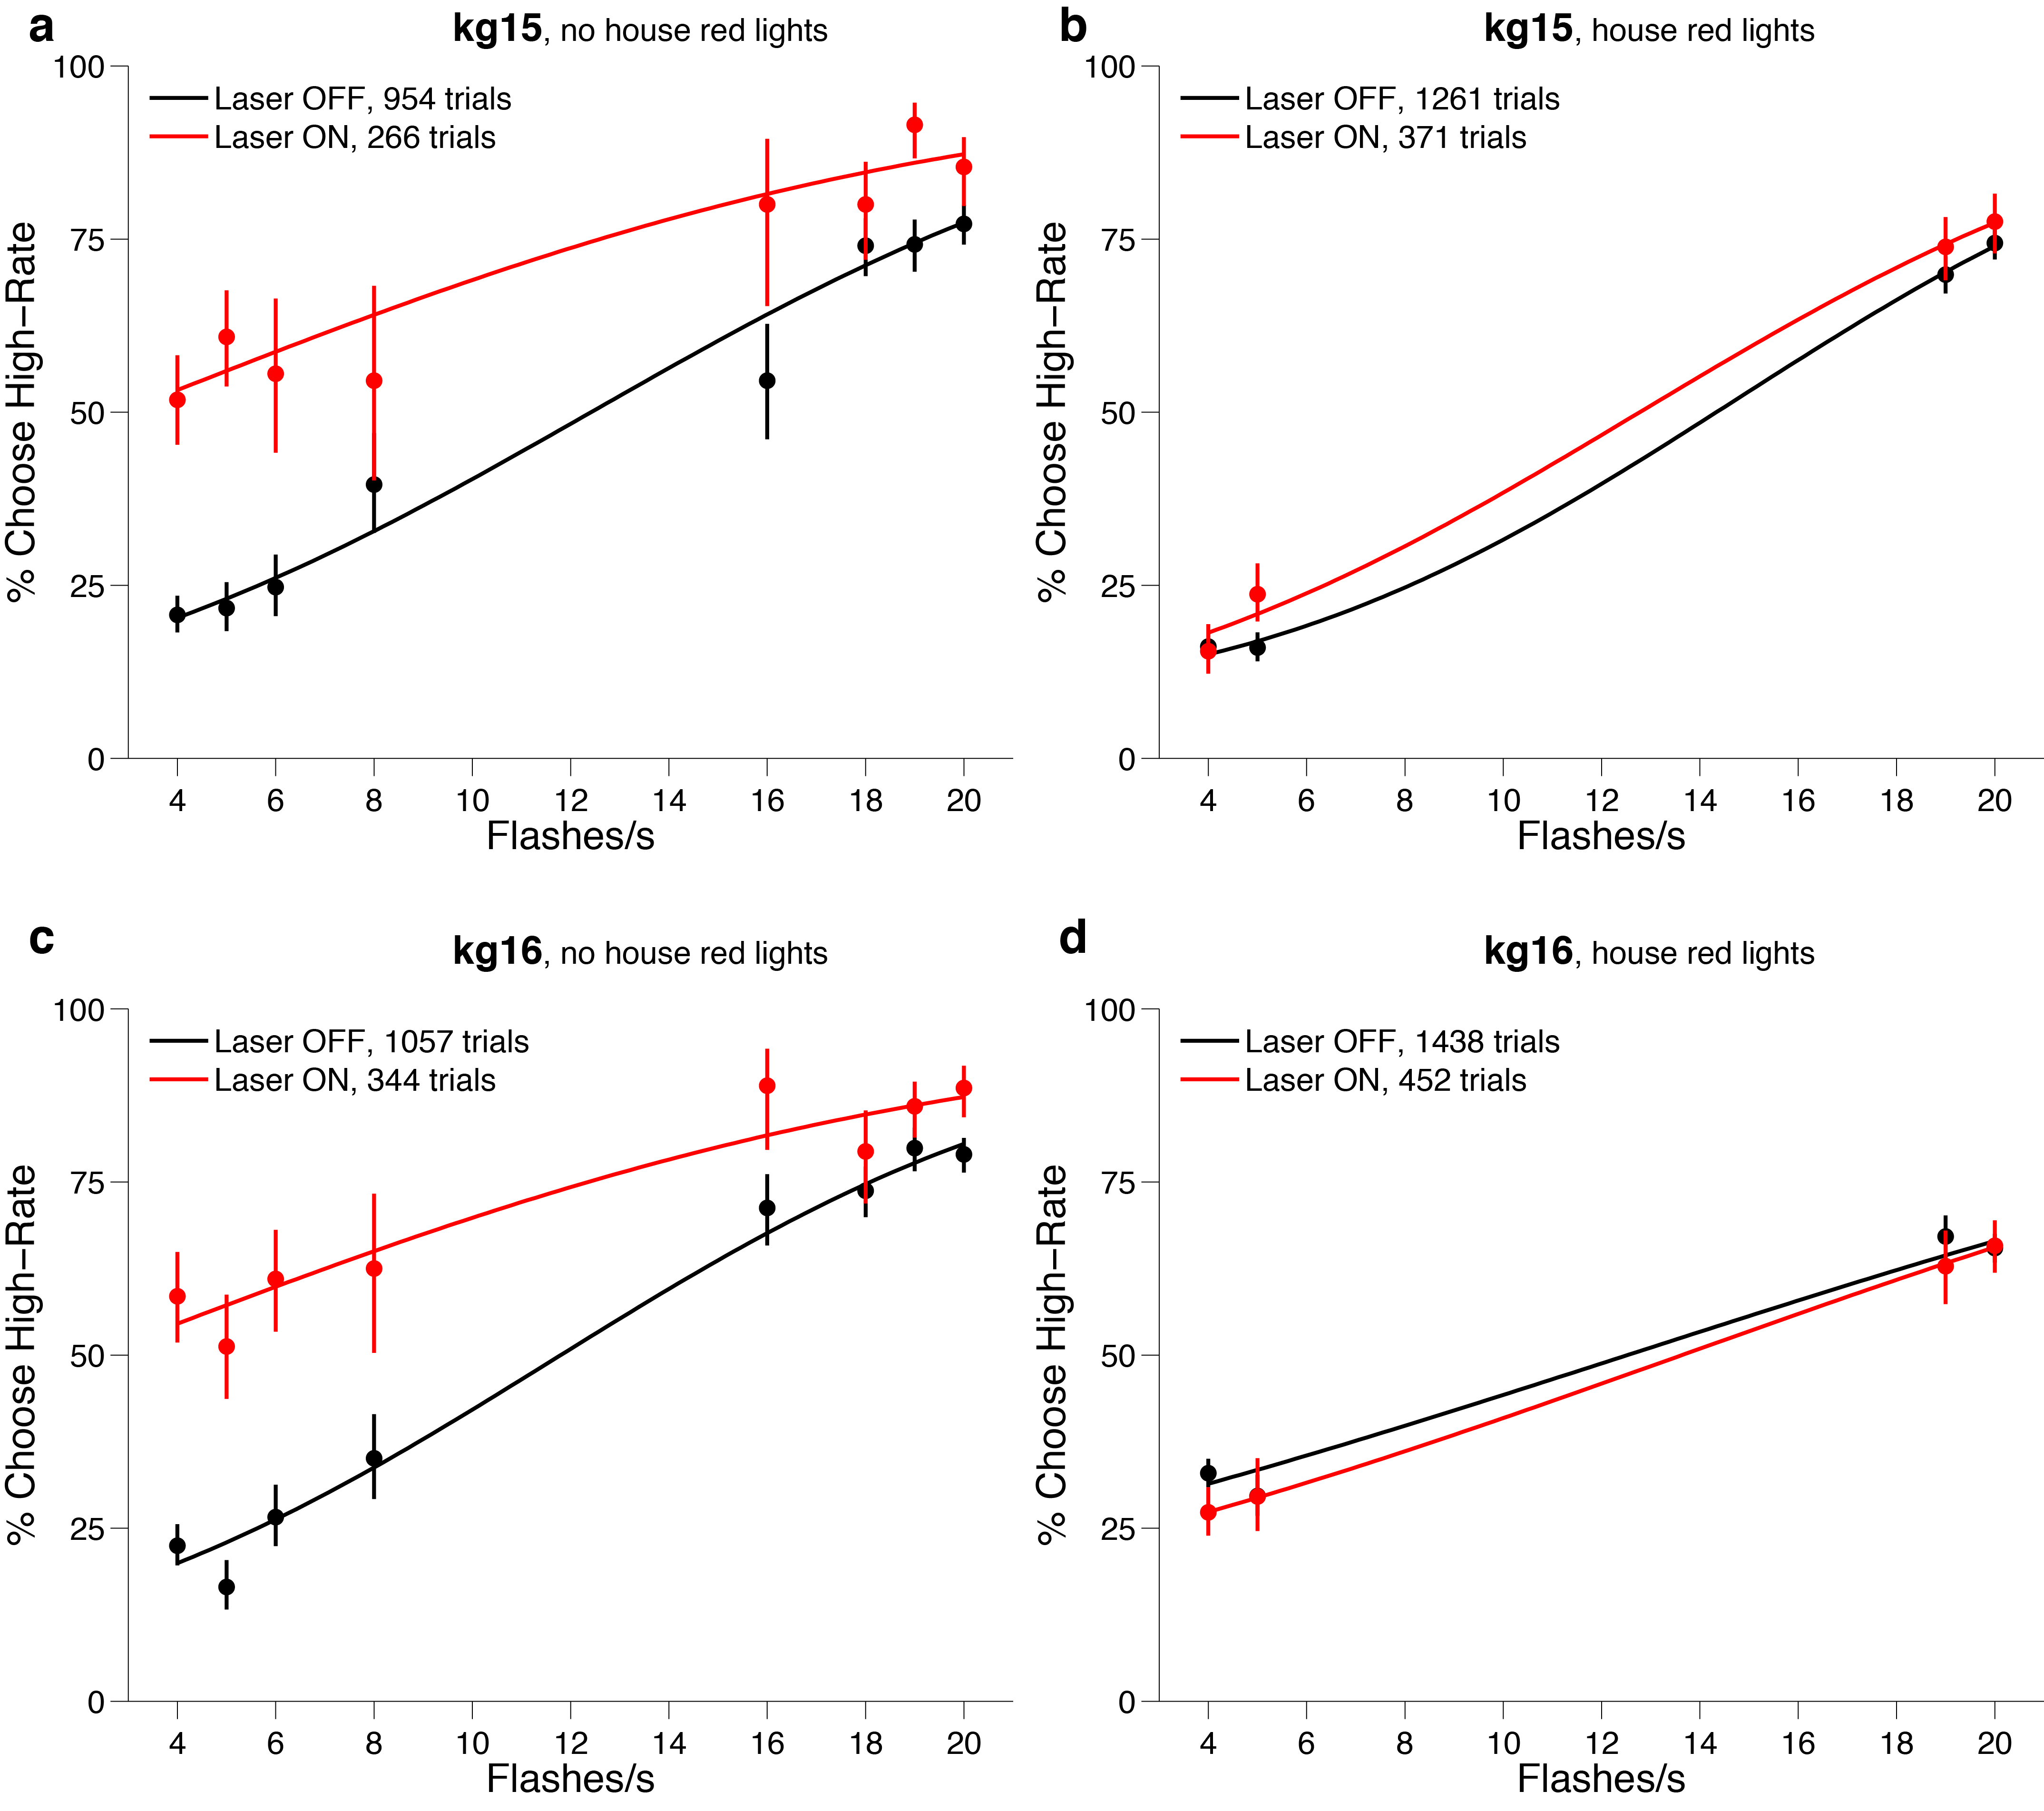
\includegraphics[width=\textwidth]{Figures/chapter4/jaws_controls_individualPMFs.png}
  \caption[Control Group Individual Psychophysical Data ]{\textbf{Control Group Individual Psychophysical Data} from two mice (kg15 and kg16) under two conditions. (a,c) Without the masking red light. Laser stimulation irradiance 32 mW/mm$^{2}$. (b,d) Masking red lights present in the behavior booth. Laser stimulation irradiance 64 mW/mm$^{2}$. Circles represent the subject's behavioral response during laser OFF (black) and laser ON (red) trials. Solid line represents the psychometric function fit to cumulative Normal (Equation \ref{eq:normalpmf}). Error bars represent Wilson Binomial (95\%) confidence intervals. }
   \label{fig:ctrlindividual}
\end{figure}
%-----------------------------------------------------------------------------
\begin{figure}
  \centering
   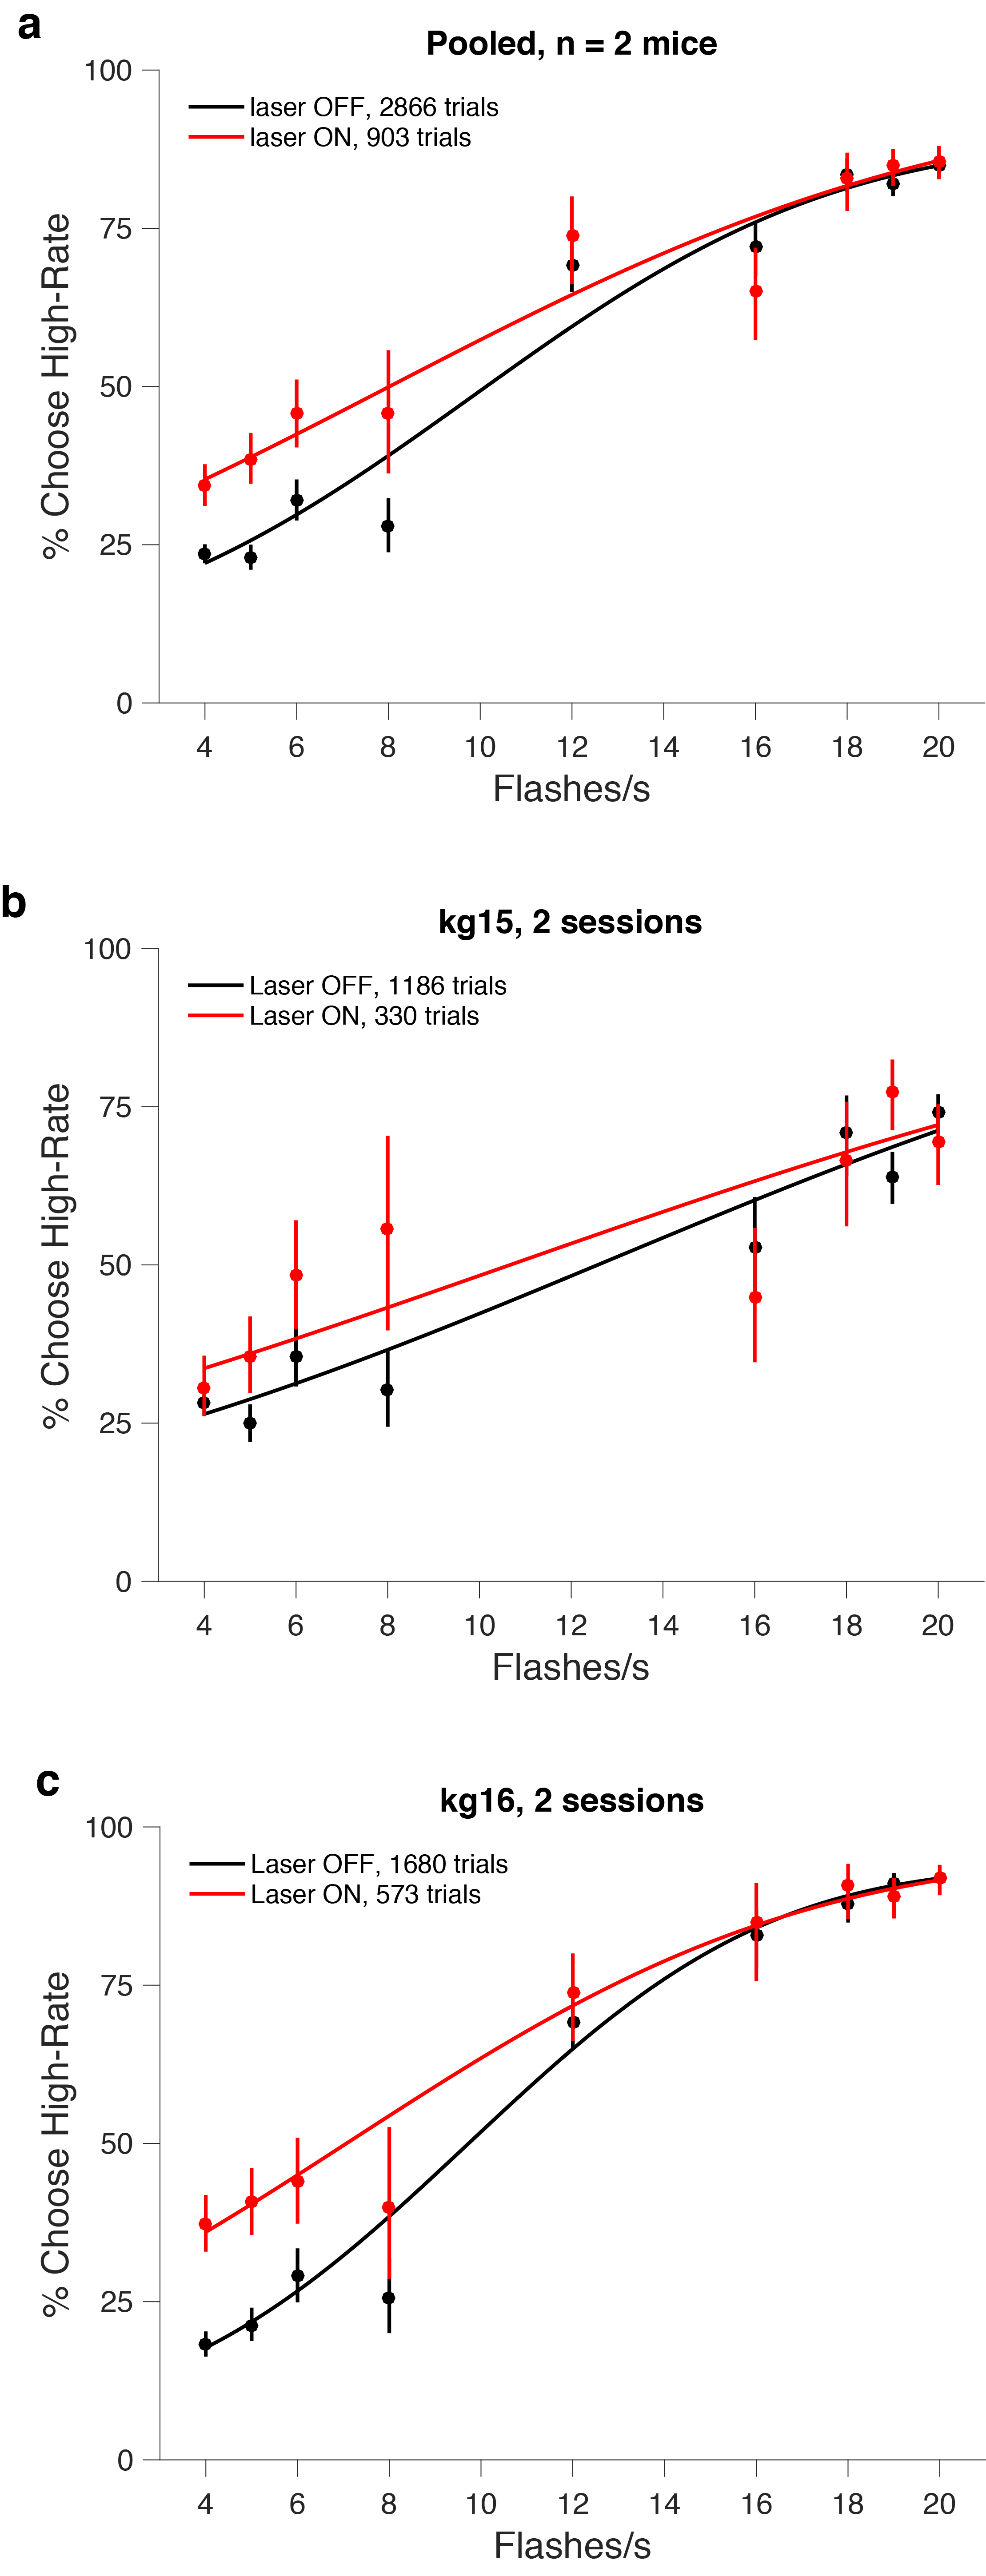
\includegraphics[width=\textwidth,height=0.75\textheight,keepaspectratio]{Figures/chapter4/jaws_controls_house_red_full_rates_PMFs.png}
  \caption[Control Group Psychophysical Data - More Flash Rates]{\textbf{Control Group Psychophysical Data - More Flash Rates} (a) Pooled psychophysical data from two mice (b) kg15 and (c) kg16 with more flash rates. Masking red light present during sessions. Laser stimulation irradiance at 64 mW/mm$^{2}$. Solid line represents the psychometric function fit to cumulative Normal (Equation \ref{eq:normalpmf}). Error bars represent Wilson Binomial (95\%) confidence intervals. }
   \label{fig:ctrlpmfs}
\end{figure}
%-----------------------------------------------------------------------------
\begin{figure}
  \centering
   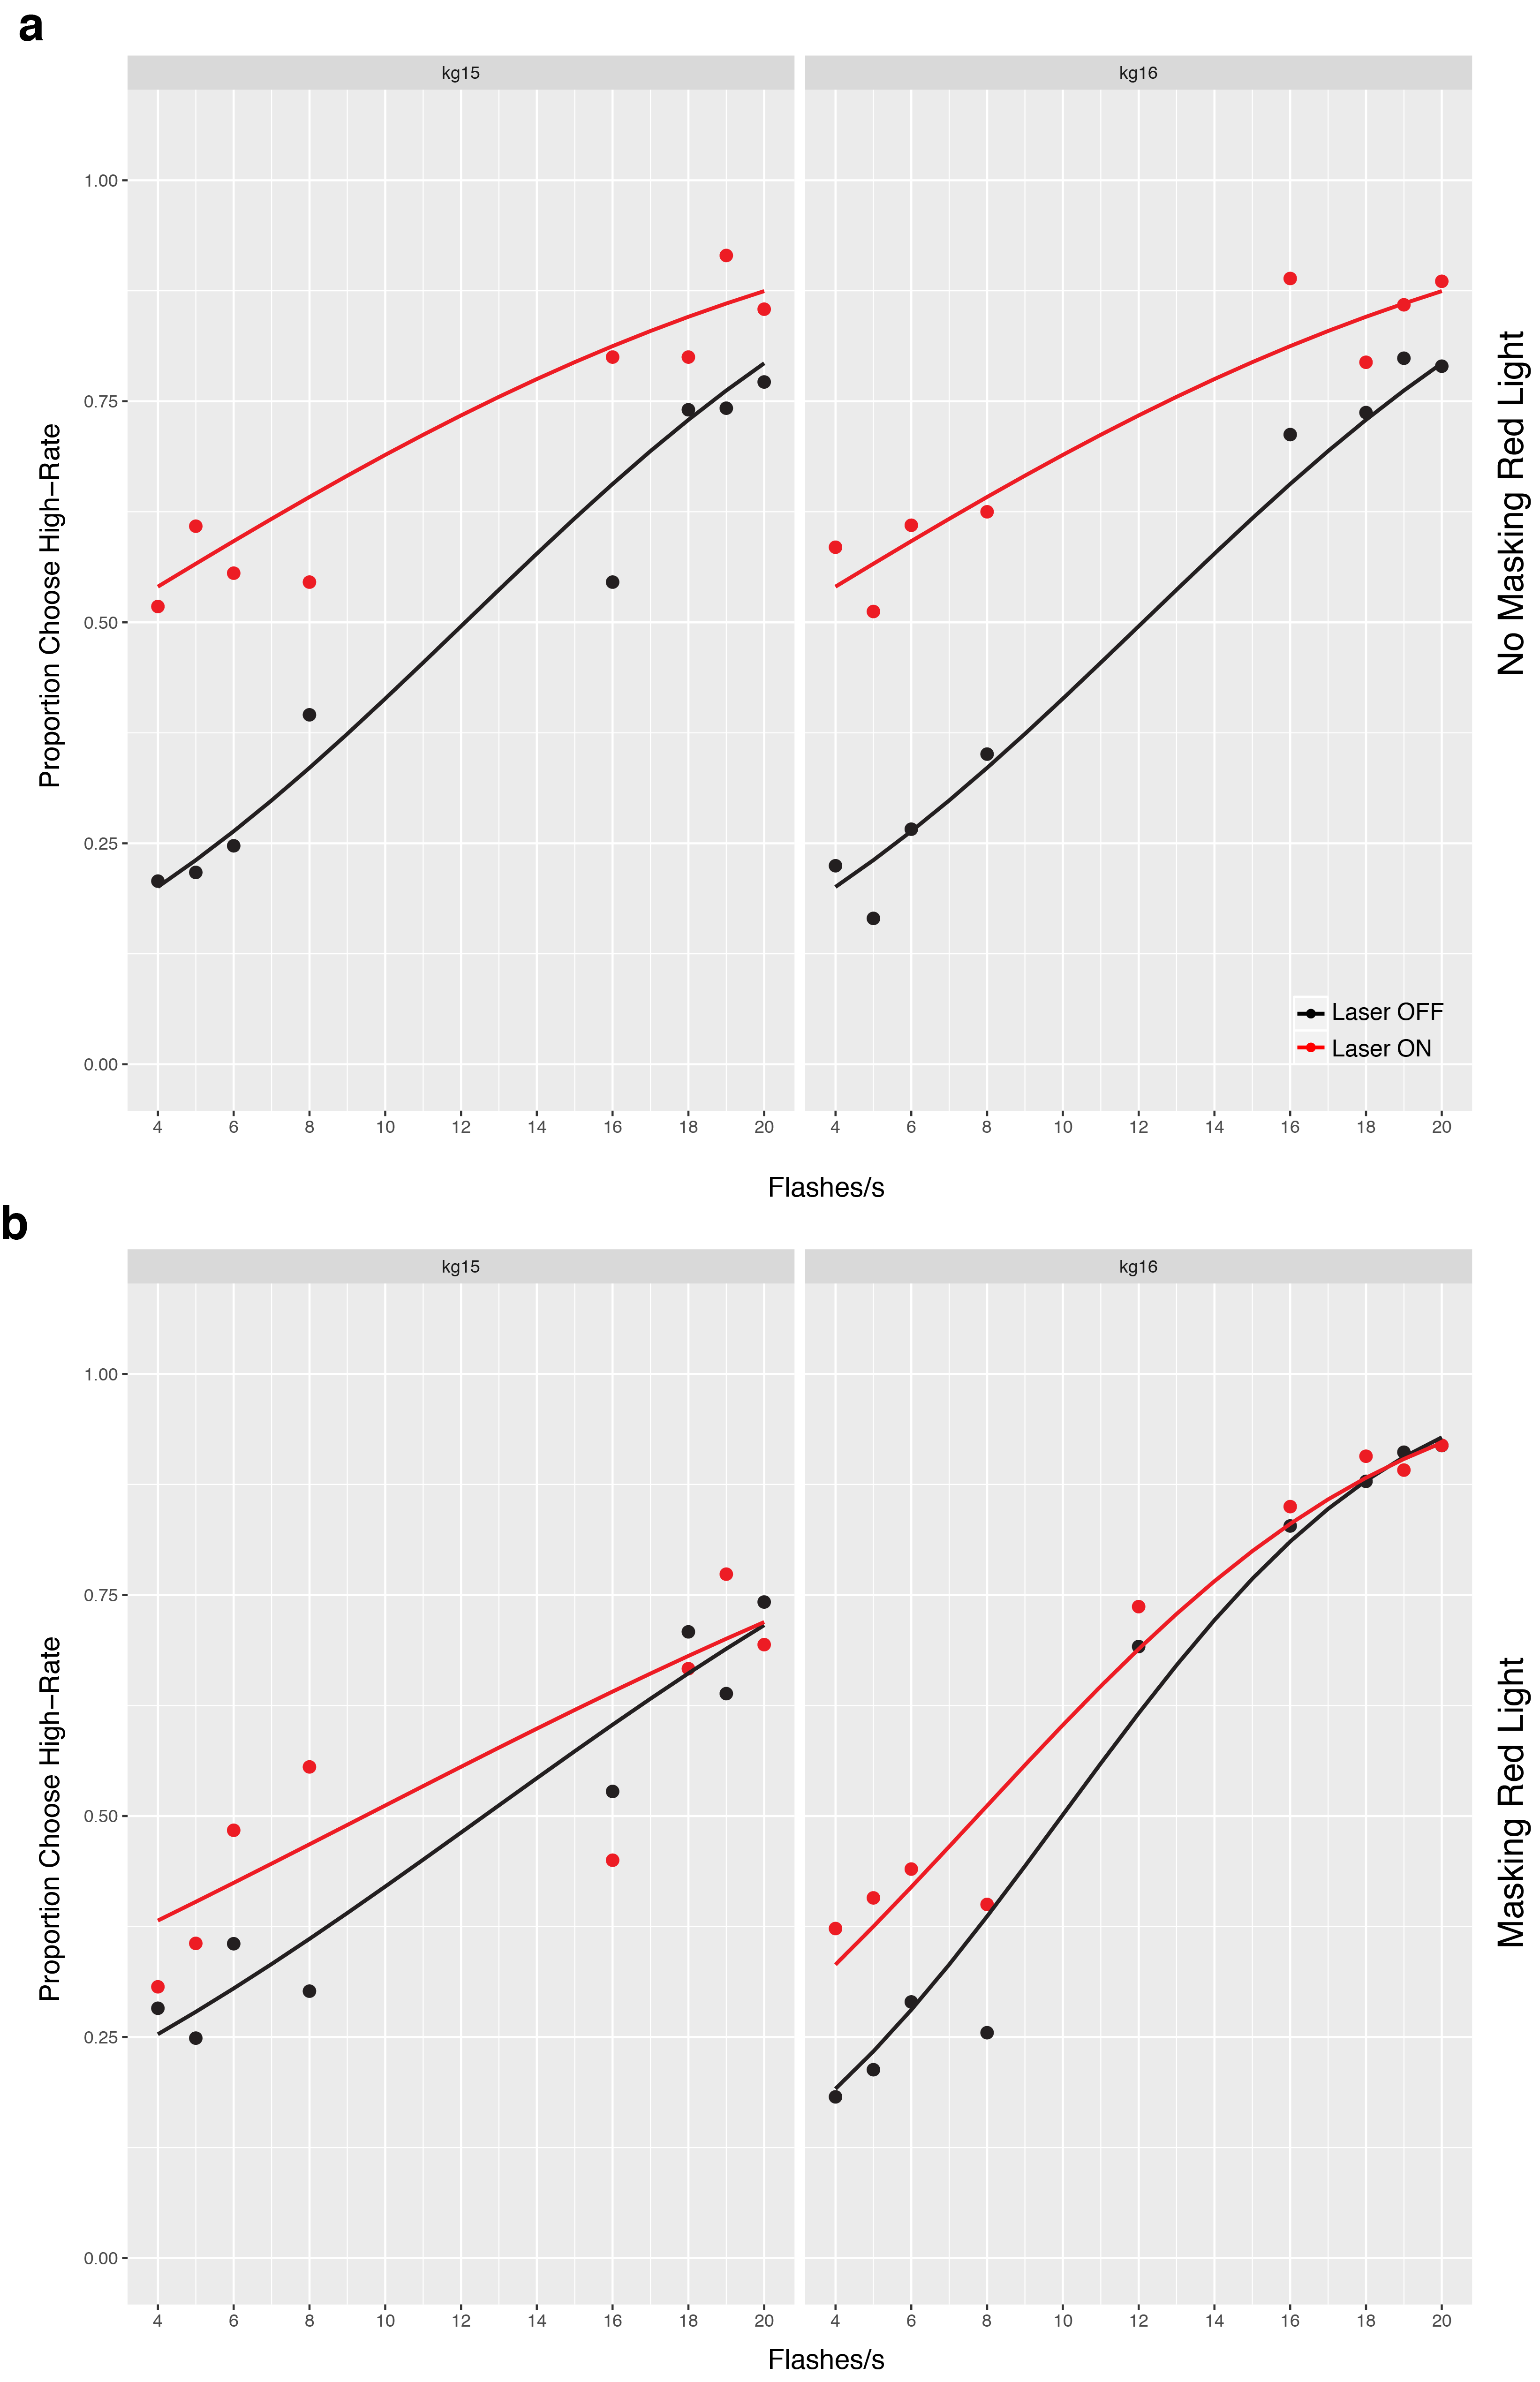
\includegraphics[width=\textwidth,height=0.8\textheight,keepaspectratio]{Figures/chapter4/GLMM_PMFS_controls.png}
  \caption[Psychometric GLMM Fit - Control Group]{\textbf{Psychometric GLMM Fit - Control Group} for n = 2 mice (a) No masking red light, laser stimulation at 32 mW/mm$^{2}$ (b) Masking red light present, laser stimulation irradiance at 64 mW/mm$^{2}$. Circles represent the subject's response data for laser OFF (black) and laser ON (red) conditions. The solid line represents the GLMM fit. }
   \label{fig:glmmcontrolpmfs}
\end{figure}

%-----------------------------------------------------------------------------
\begin{figure}
  \centering
   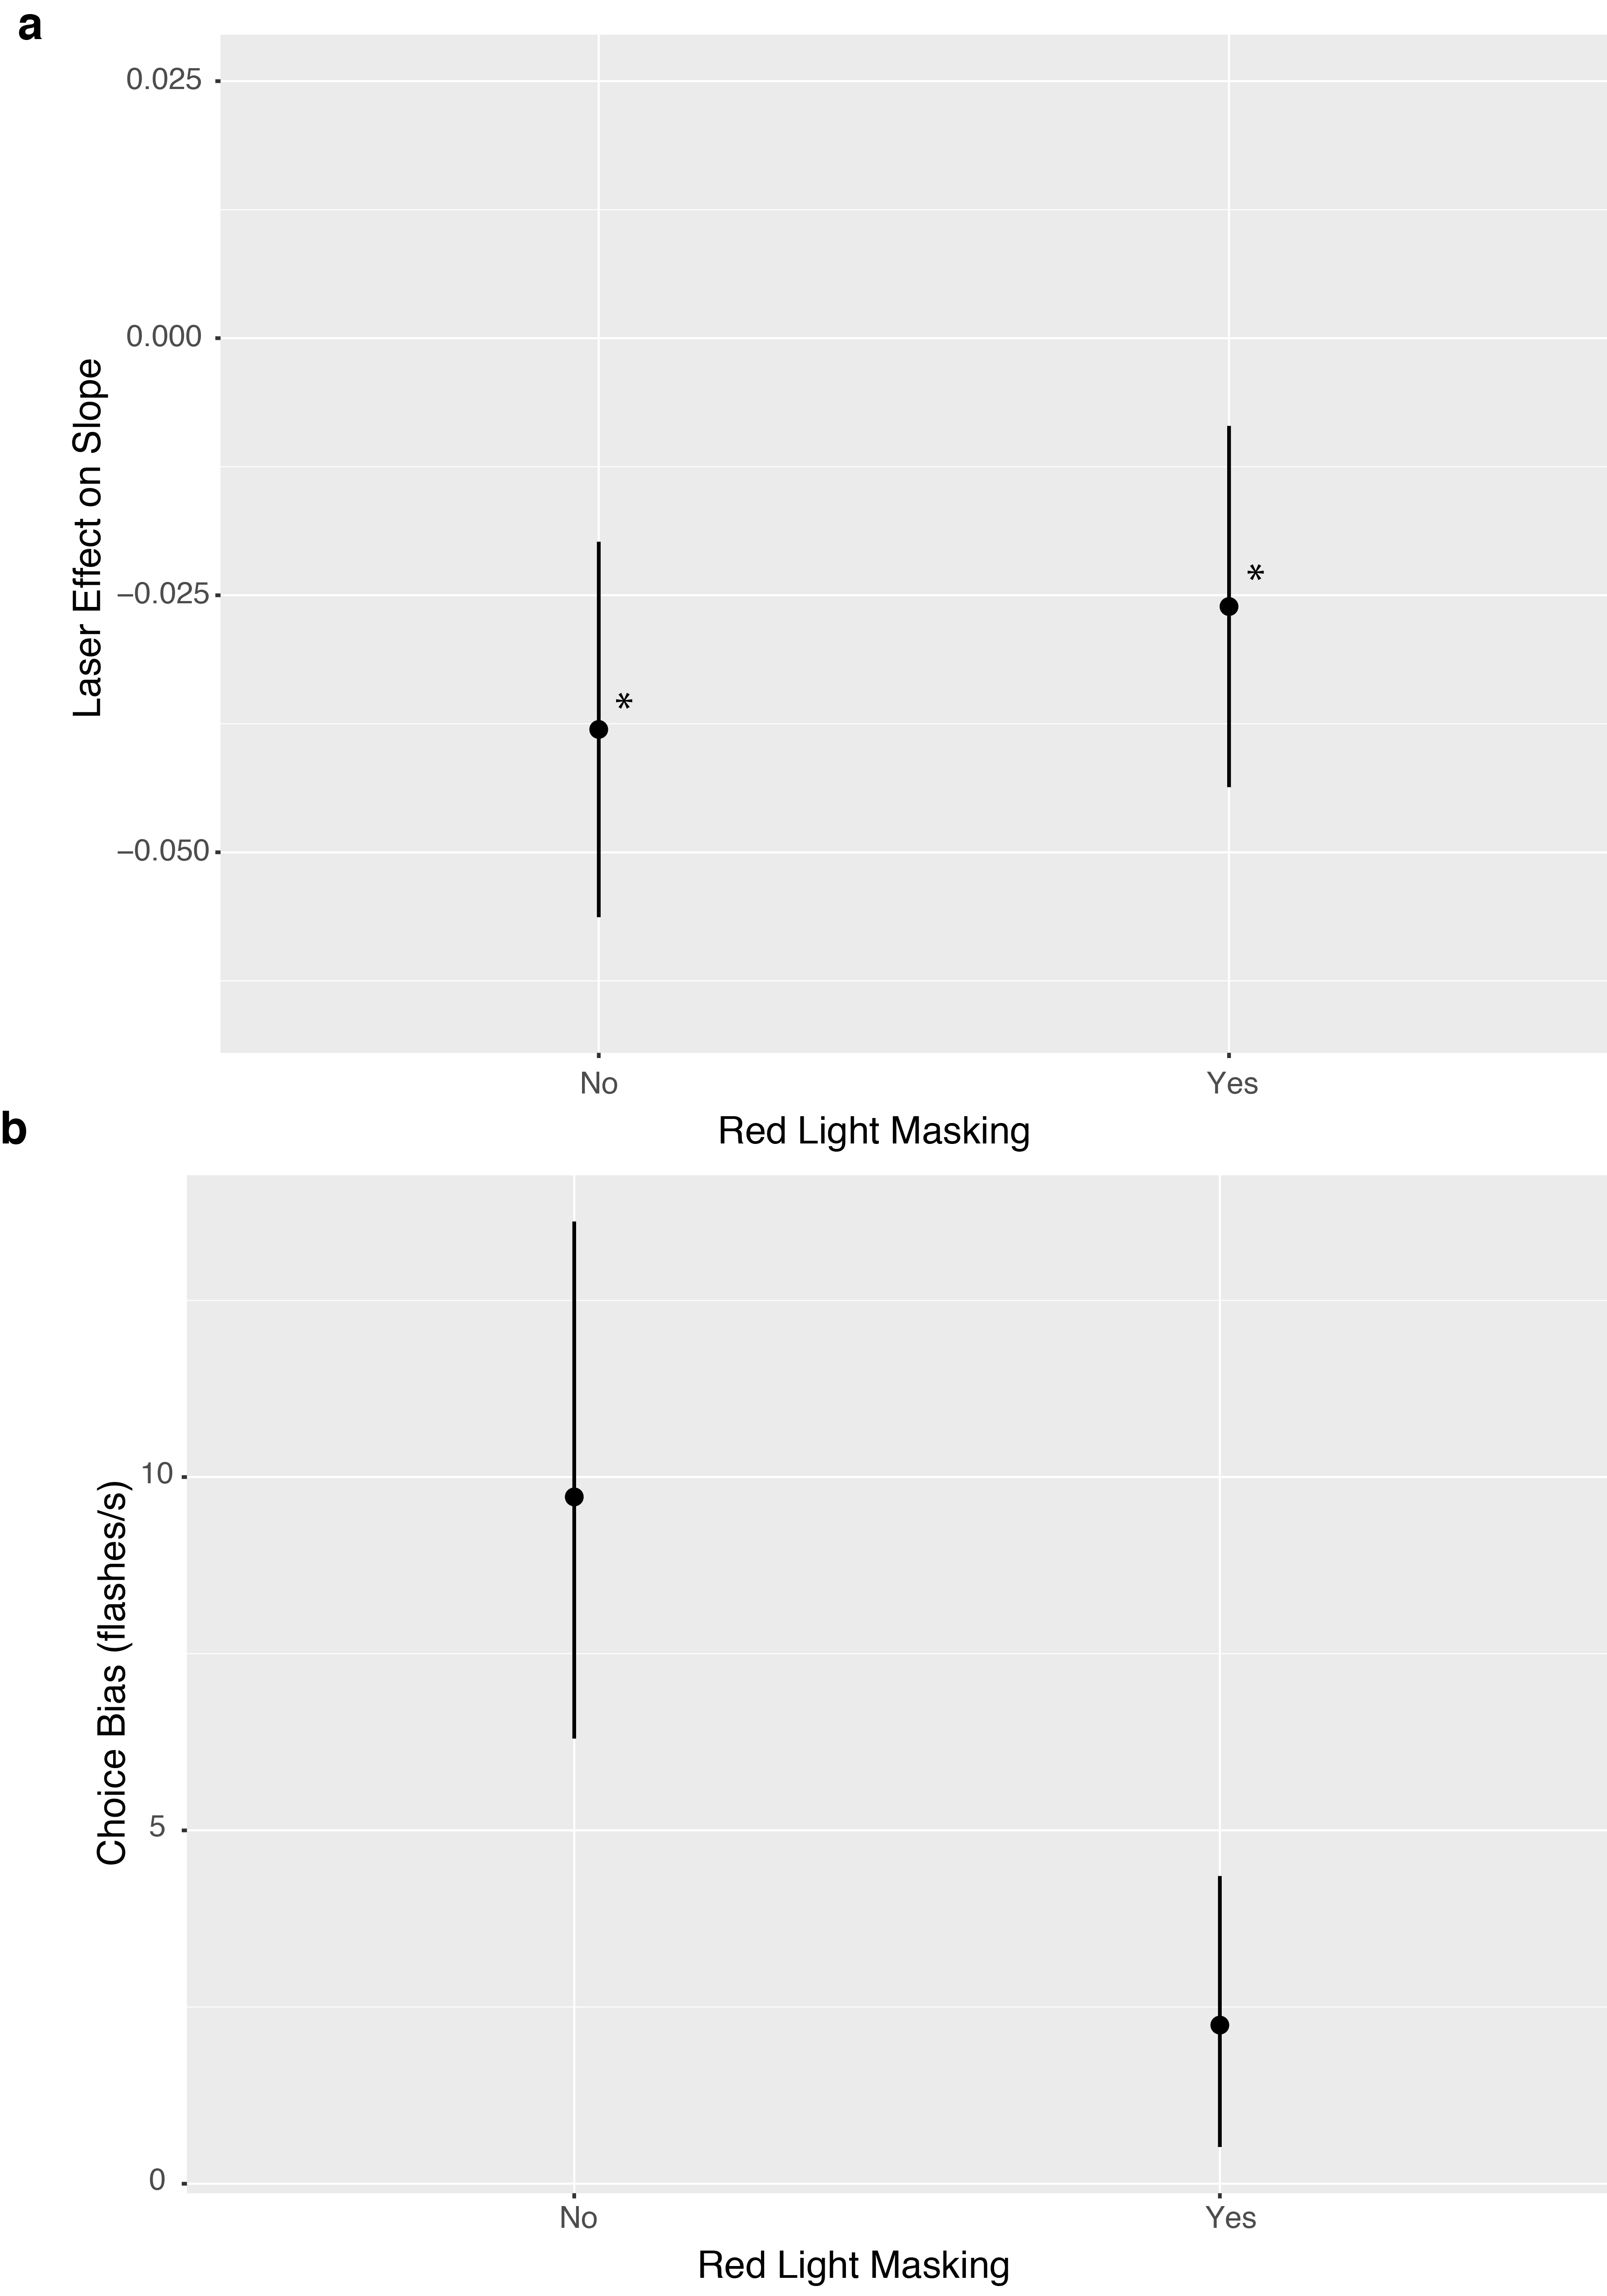
\includegraphics[width=\textwidth,height=0.8\textheight,keepaspectratio]{Figures/chapter4/glmm_pmf_effects_controls.png}
  \caption[Psychophysical Effects of \emph{in vivo} red light stimulation on control group]{\textbf{Psychophysical Effects of \emph{in vivo} Red Light Stimulation - control Group} (a) Effect of \emph{in vivo} red light stimulation on the slope of the psychometric function ($\beta_{evidence:opto}$) in the presence and absence of masking red light. Irradiance for each condition is 32 and 64 mW/mm$^{2}$ respectively. Error bars represent 95\% confidence interval. Asterisks mark statistically significant (p<0.05) coefficients. (b) Choice bias as defined in Equation \ref{choicebias}. Choice bias error bars represent 95\% confidence intervals estimated by error propagation.}
   \label{fig:glmmcontrol}
\end{figure}
%-----------------------------------------------------------------------------
\begin{figure}
  \centering
   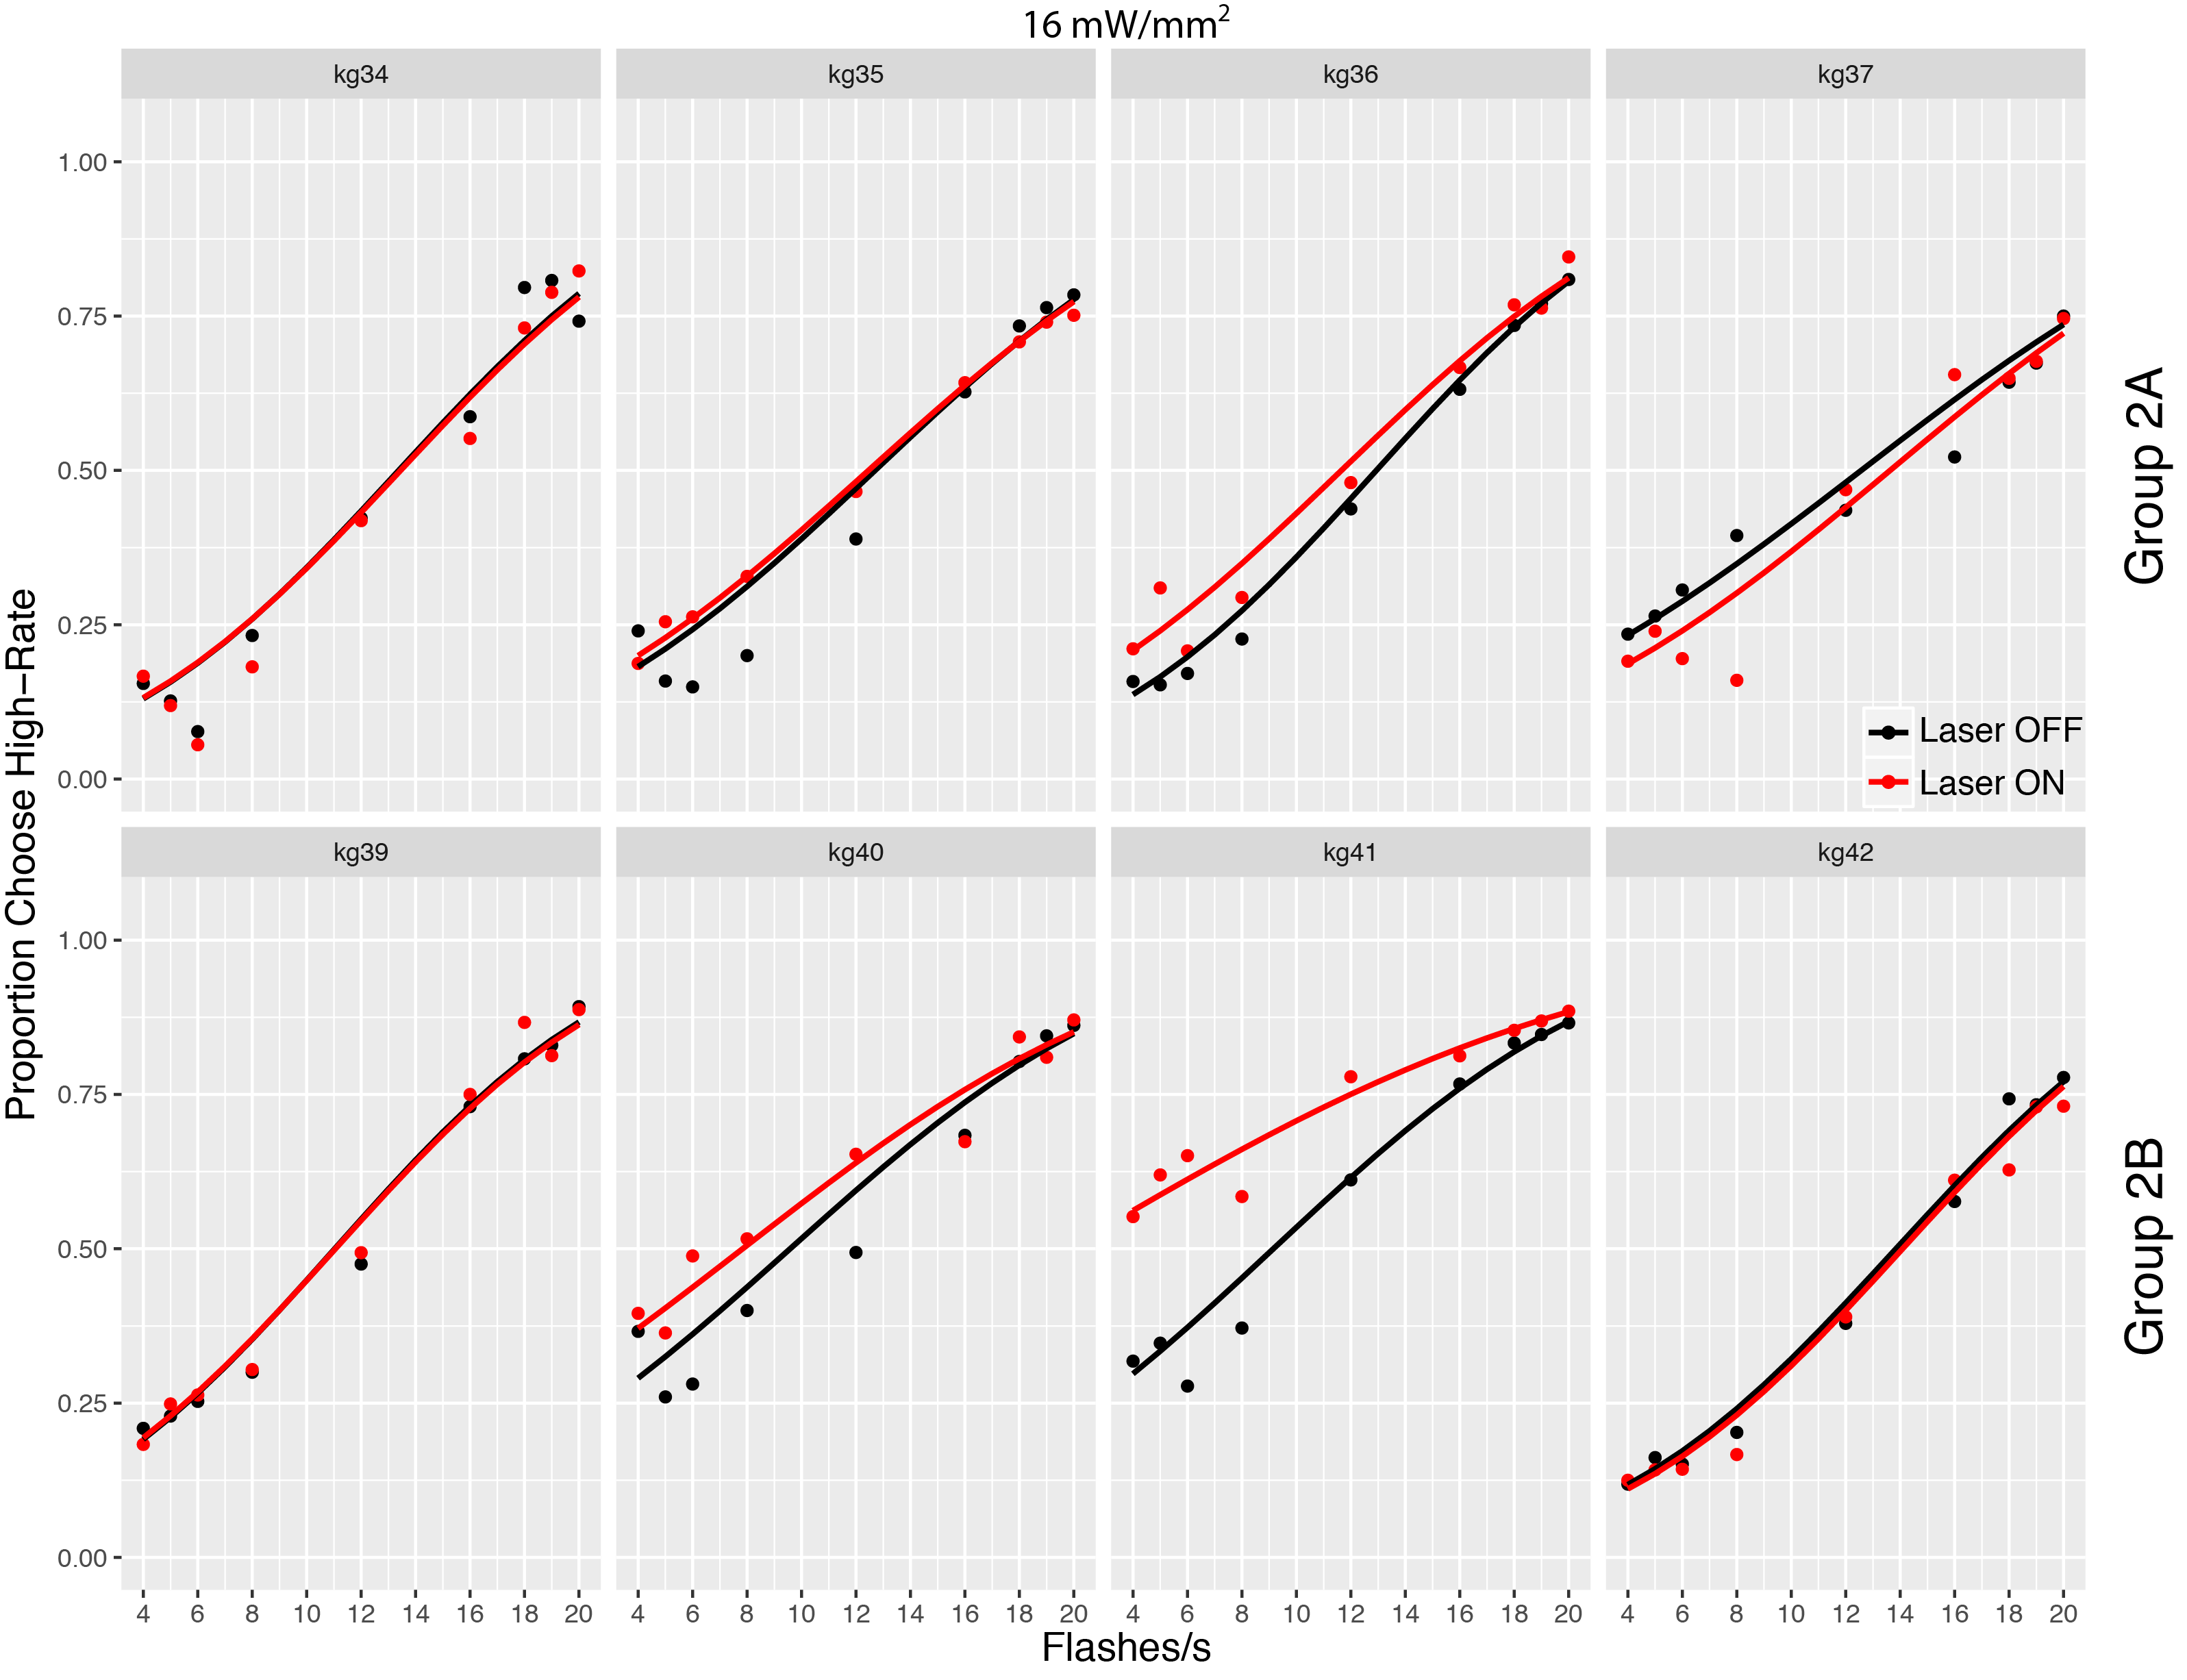
\includegraphics[width=\textwidth]{Figures/chapter4/glmm_PMFS_16mWmm2.png}
  \caption[Psychometric GLMM Fit - AM Group 2 - 16 mW/mm$^{2}$]{\textbf{Psychometric GLMM Fit - AM Group 2 - 16 mW/mm$^{2}$} for each mouse (n=8). Circles represent the subject's response data for laser OFF (black) and laser ON (red) conditions. The solid line represents the GLMM fit. Top row is group 2A and bottom row is group 2B. }
   \label{fig:amGLMM16}
\end{figure}
%-----------------------------------------------------------------------------
\begin{figure}
  \centering
   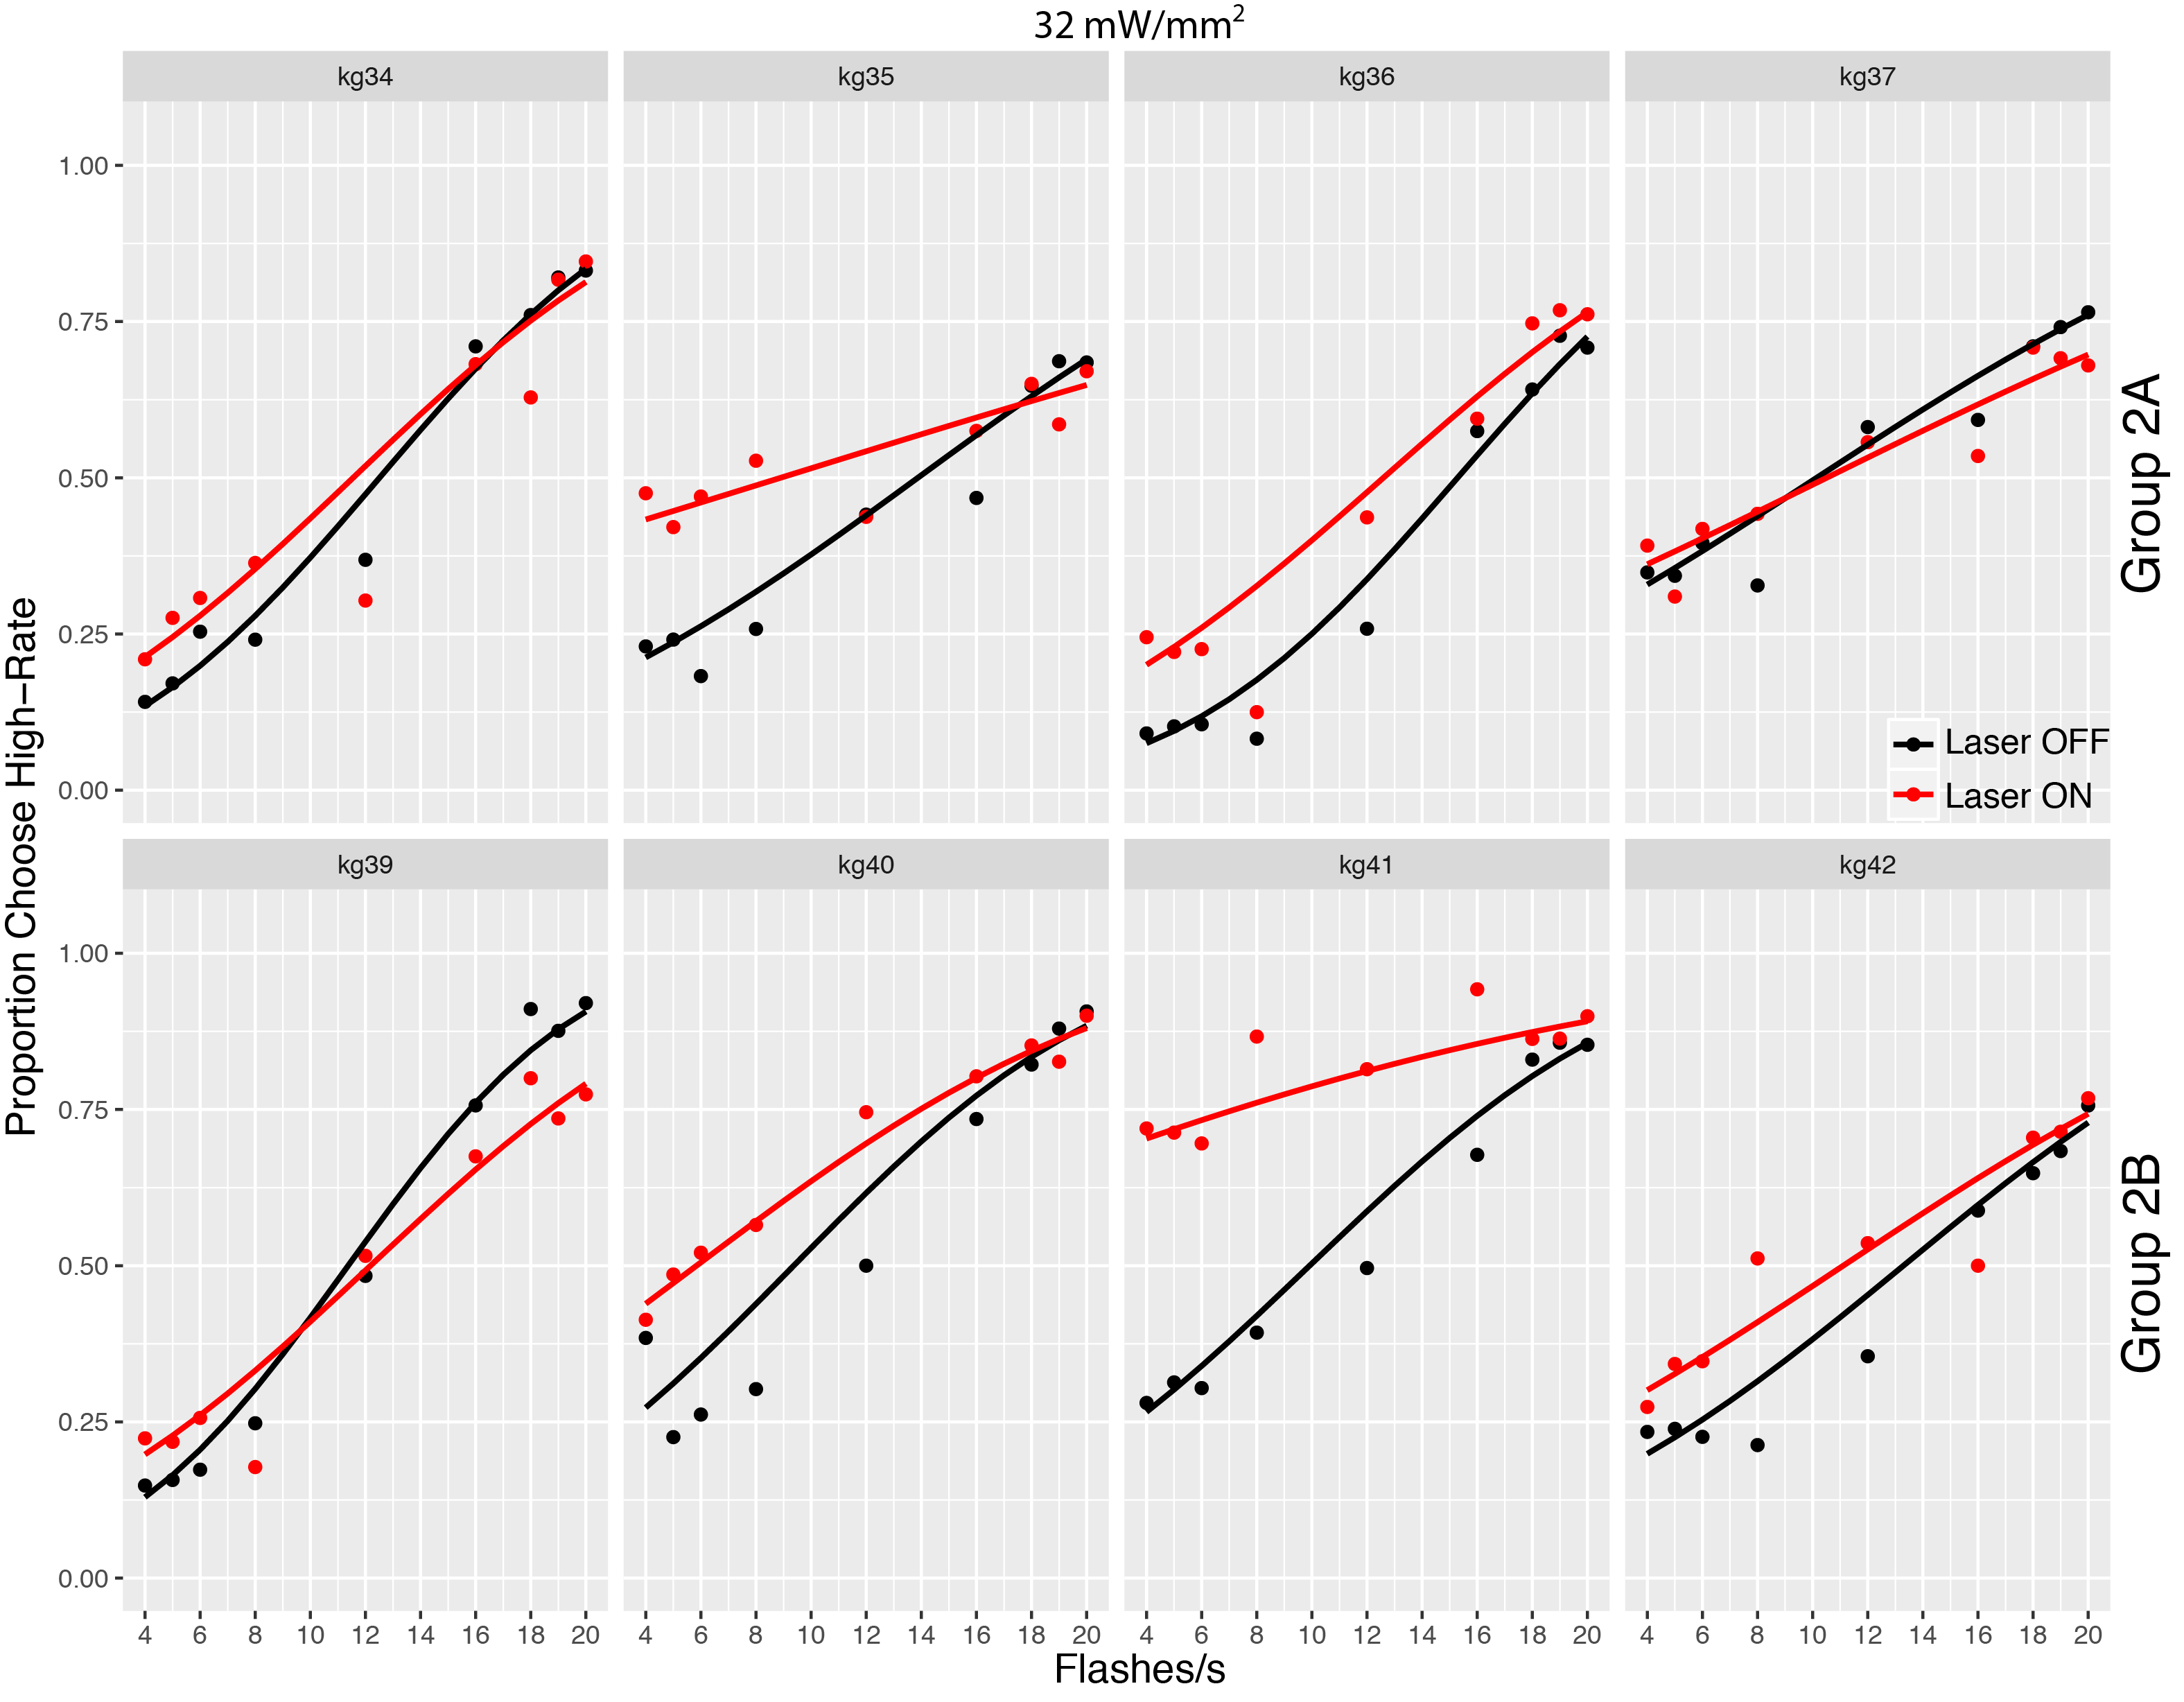
\includegraphics[width=\textwidth]{Figures/chapter4/glmm_PMFS_32mWmm2.png}
  \caption[Psychometric GLMM Fit - AM Group 2 - 32 mW/mm$^{2}$]{\textbf{Psychometric GLMM Fit- AM Group 2 - 32 mW/mm$^{2}$} for each mouse (n=8). Circles represent the subject's response data for laser OFF (black) and laser ON (red) conditions. The solid line represents the GLMM fit. Top row is group 2A and bottom row is group 2B.}
   \label{fig:amGLMM32}
\end{figure}
%-----------------------------------------------------------------------------
\begin{figure}
  \centering
   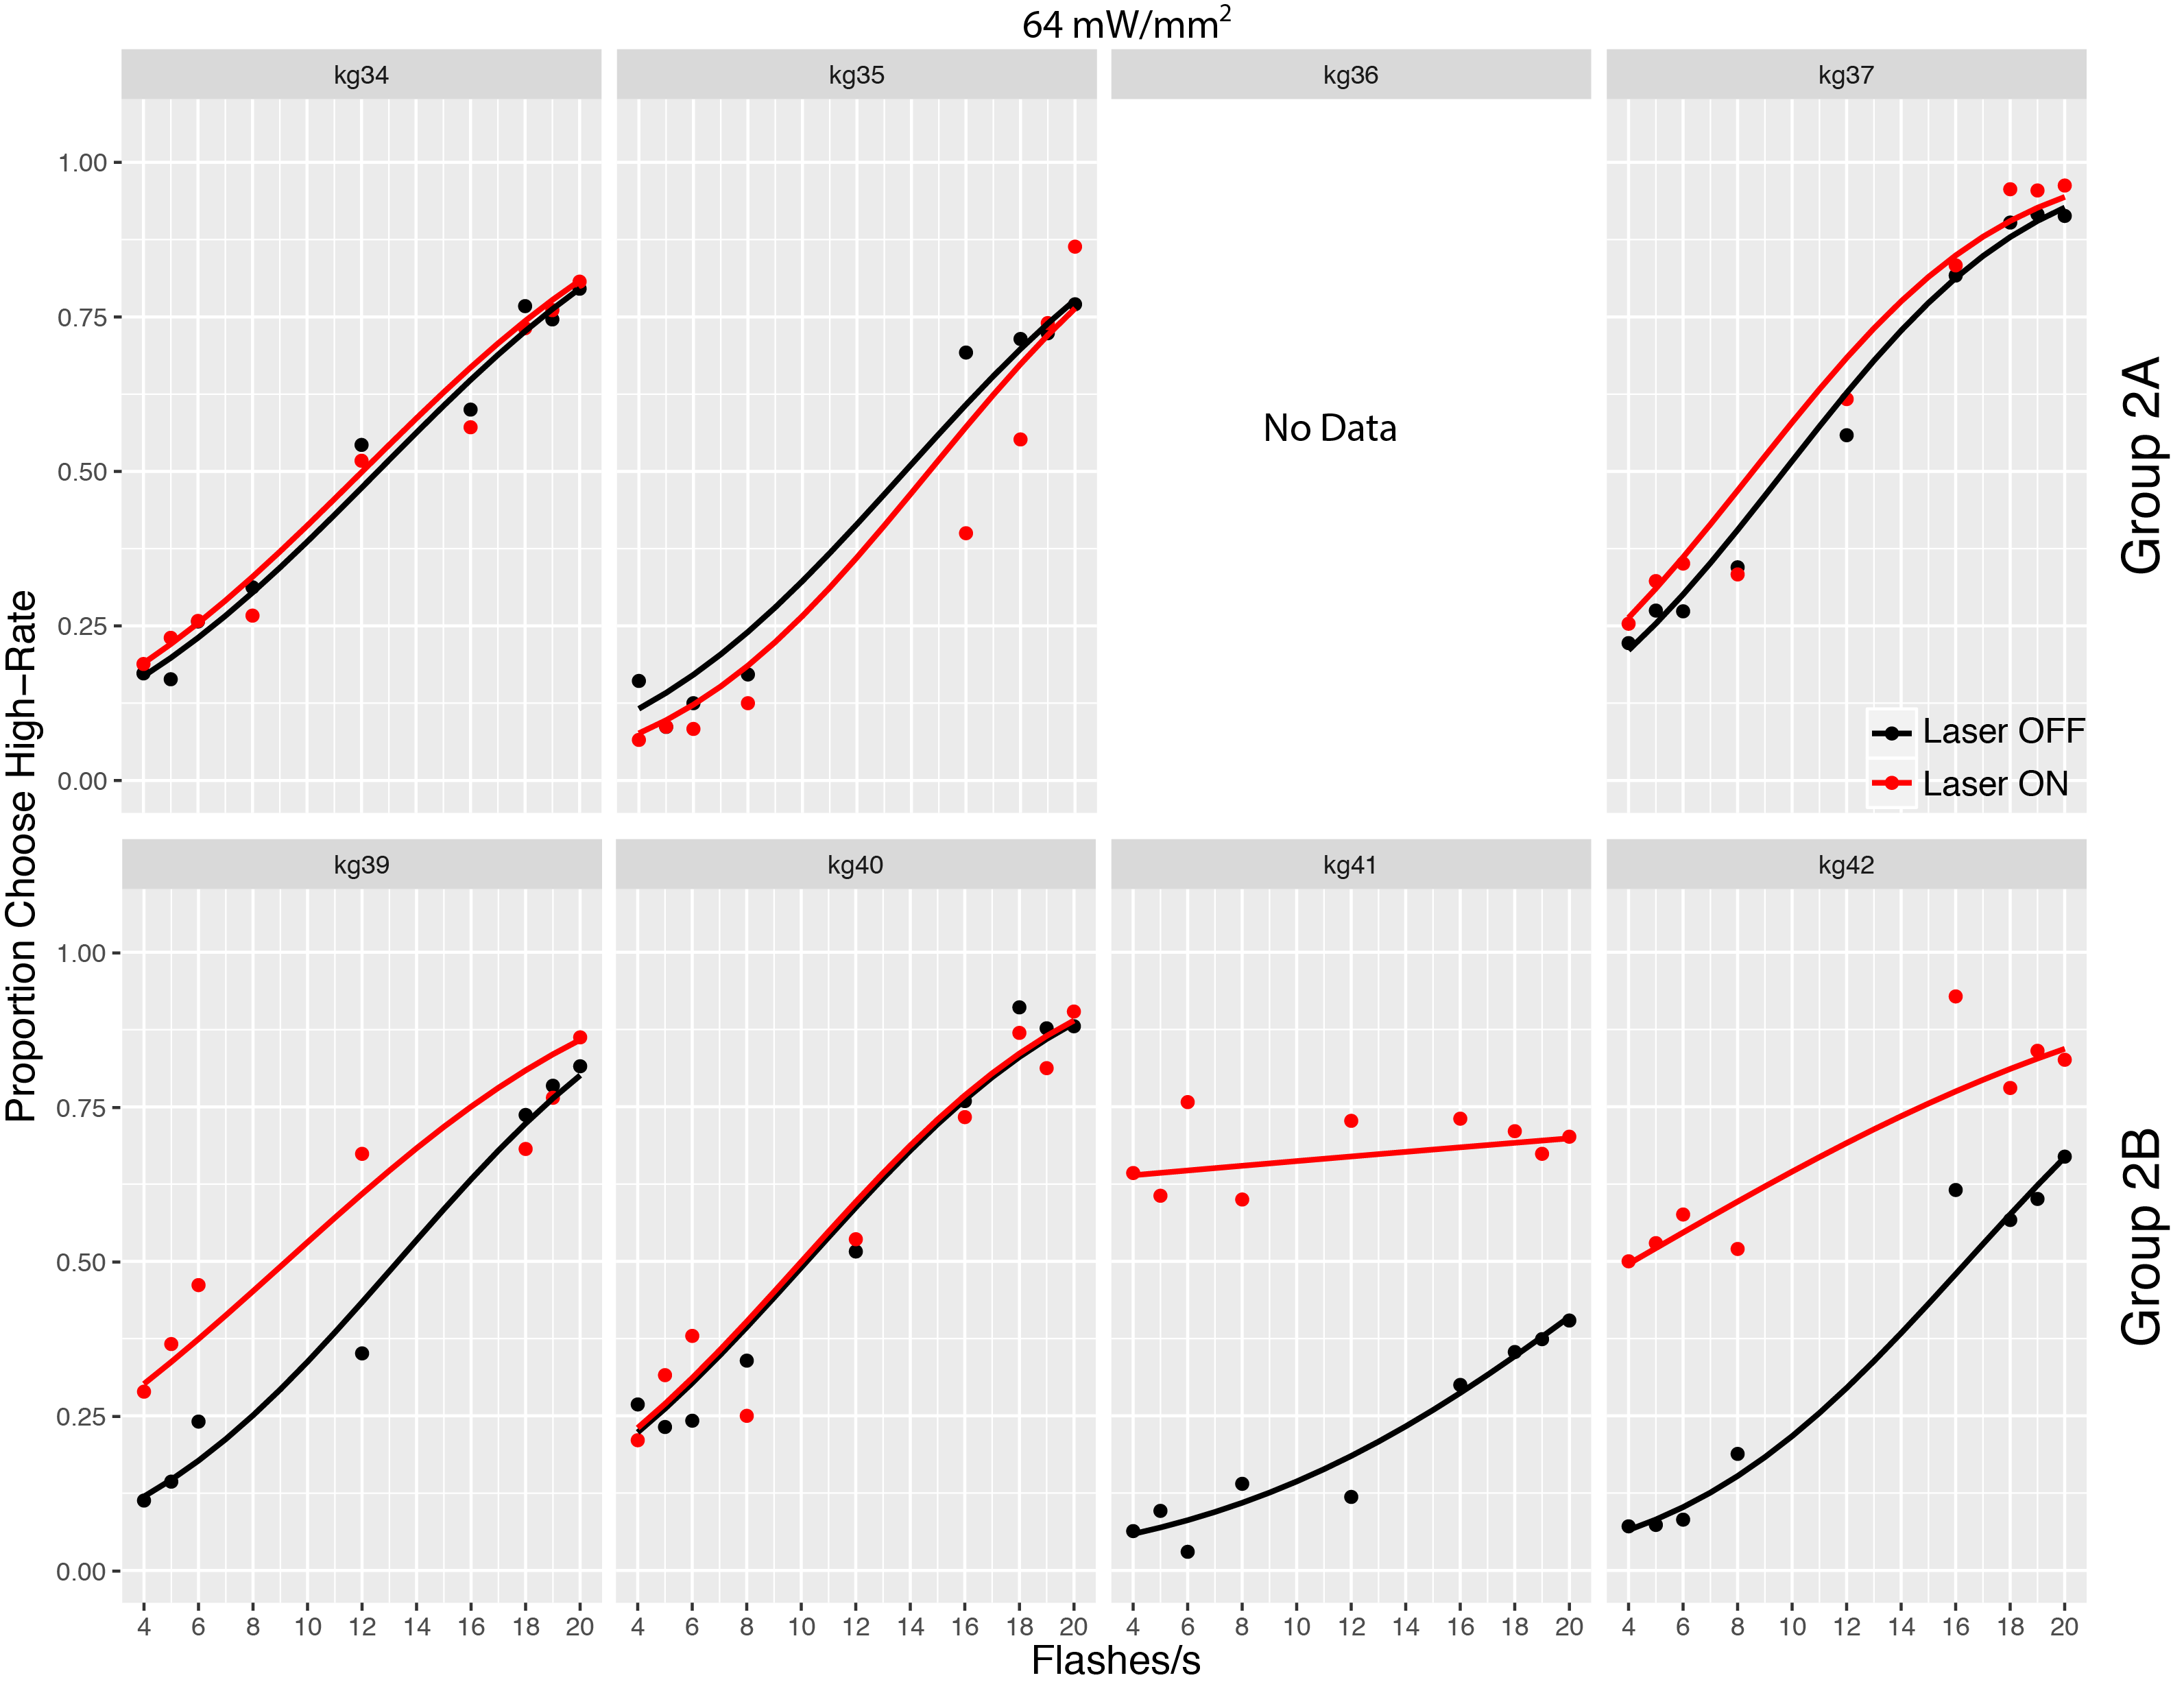
\includegraphics[width=\textwidth]{Figures/chapter4/glmm_PMFS_64mWmm2.png}
  \caption[Psychometric GLMM Fit - AM Group 2 - 64 mW/mm$^{2}$]{\textbf{Psychometric GLMM Fit - AM Group 2 - 64 mW/mm$^{2}$} for each mouse (n=7). Circles represent the subject's response data for laser OFF (black) and laser ON (red) conditions. The solid line represents the GLMM fit. Top row is group 2A and bottom row is group 2B. }
   \label{fig:amGLMM64}
\end{figure}
%-----------------------------------------------------------------------------






